% Báo cáo kỹ thuật sơ bộ: Soi - đọc và kiểm chứng BCTC Việt Nam
% Định dạng theo mẫu báo cáo Project III của Trường CNTT&TT, ĐHBK Hà Nội (lớp report 12pt, lề 2,5 cm, giãn dòng 1,5,
% phông Computer Modern/Latin Modern, tài liệu tham khảo BibTeX kiểu plain).
% Biên dịch: xelatex main -> bibtex main -> xelatex main -> xelatex main  (hoặc: latexmk -xelatex main.tex)
\documentclass[12pt,a4paper]{report}

% ============================================================================
% PACKAGES
% ============================================================================
\usepackage{fontspec}               % XeLaTeX: phông Latin Modern (giống Computer Modern, đủ dấu tiếng Việt)
\usepackage[vietnamese]{babel}
\usepackage{amsmath,amssymb,amsfonts}
\usepackage{graphicx}
\usepackage{booktabs}
\usepackage{longtable}
\usepackage{array}
\usepackage{tabularx}
\usepackage{multirow}
\usepackage{algorithm}
\usepackage[noend]{algpseudocode}
\usepackage{listings}               % chỉ dùng bộ đếm và tên "Đoạn mã"; khối mã viết bằng fancyvrb (đúng chữ có dấu)
\usepackage{fancyvrb}
\usepackage[table]{xcolor}
\usepackage{hyperref}
\usepackage{geometry}
\usepackage{setspace}
\usepackage{caption}
\usepackage{subcaption}
\usepackage{float}
\usepackage{enumitem}
\usepackage{url}
\usepackage{tcolorbox}
\usepackage{tikz}
\usetikzlibrary{arrows.meta,positioning,shapes.geometric,shapes.misc,calc}
\usepackage{pgfplots}
\pgfplotsset{compat=1.18}

\geometry{margin=2.5cm}
\onehalfspacing
\graphicspath{{hinh/}}
\setcounter{tocdepth}{2}
\hypersetup{hidelinks}
\setlist{itemsep=1pt,topsep=3pt}

\newcommand{\enquote}[1]{“#1”}
\newcommand{\code}[1]{\texttt{#1}}
\newcommand{\chualam}{\par\noindent\textit{(Dự kiến, chưa thực hiện.)}\par}

\renewcommand{\lstlistingname}{Đoạn mã}

\algrenewcommand\algorithmicrequire{\textbf{Vào:}}
\algrenewcommand\algorithmicensure{\textbf{Ra:}}
\algrenewcommand\algorithmicfor{\textbf{với mỗi}}
\algrenewcommand\algorithmicdo{\textbf{làm}}
\algrenewcommand\algorithmicif{\textbf{nếu}}
\algrenewcommand\algorithmicthen{\textbf{thì}}
\algrenewcommand\algorithmicelse{\textbf{ngược lại}}
\algrenewcommand\algorithmicreturn{\textbf{trả về}}
\floatname{algorithm}{Thuật toán}

% Màu dùng trong sơ đồ
\definecolor{soiblue}{RGB}{18,92,173}
\definecolor{soigreen}{RGB}{46,140,87}
\definecolor{soiamber}{RGB}{214,140,20}
\definecolor{soired}{RGB}{190,50,50}
\definecolor{soigray}{RGB}{110,116,128}
\definecolor{lightblue}{RGB}{228,239,252}
\definecolor{lightgreen}{RGB}{224,244,232}
\definecolor{lightamber}{RGB}{255,241,214}
\definecolor{lightred}{RGB}{252,226,226}
\definecolor{lightgray}{RGB}{242,243,245}

% Hộp ghi chú: khung mảnh, nền xám nhạt, hợp văn phong báo cáo
\newtcolorbox{ghichu}[1]{colback=lightgray,colframe=black!55,boxrule=0.4pt,arc=0pt,
  fonttitle=\bfseries,coltitle=black,colbacktitle=black!10,title=#1}

\tikzset{
  box/.style={draw=soiblue,fill=lightblue,rounded corners=3pt,align=center,font=\small\sffamily,
              minimum height=9mm,inner sep=4pt,text width=#1},
  box/.default=28mm,
  gbox/.style={box=#1,draw=soigreen,fill=lightgreen},
  gbox/.default=28mm,
  abox/.style={box=#1,draw=soiamber,fill=lightamber},
  abox/.default=28mm,
  rbox/.style={box=#1,draw=soired,fill=lightred},
  rbox/.default=28mm,
  db/.style={cylinder,shape border rotate=90,aspect=0.18,draw=soiblue,fill=lightblue,
             align=center,font=\small\sffamily,minimum height=13mm,text width=24mm},
  dec/.style={diamond,aspect=2.2,draw=soiamber,fill=lightamber,align=center,font=\small\sffamily,inner sep=1pt},
  arr/.style={-{Stealth[length=2.6mm]},thick,color=soigray},
  lab/.style={font=\scriptsize\sffamily,color=soigray,fill=white,inner sep=1pt},
  uc/.style={ellipse,draw=soiblue,fill=lightblue,align=center,font=\footnotesize\sffamily,
             minimum width=40mm,minimum height=9mm,inner sep=1pt},
  actor/.pic={\draw[thick] (0,0.42) circle (0.16);
              \draw[thick] (0,0.26) -- (0,-0.12) (-0.28,0.14) -- (0.28,0.14) (0,-0.12) -- (-0.2,-0.46) (0,-0.12) -- (0.2,-0.46);},
  life/.style={draw=soiblue,fill=lightblue,rounded corners=2pt,font=\footnotesize\sffamily,align=center,
               minimum width=20mm,minimum height=8mm},
  msg/.style={-{Stealth[length=2mm]},thick},
  ret/.style={-{Stealth[length=2mm]},dashed,color=soigray},
}

% ============================================================================
% DOCUMENT BEGIN
% ============================================================================
\begin{document}

% ============================================================================
% TRANG BÌA (theo mẫu Project III của Trường CNTT&TT)
% ============================================================================
\begin{titlepage}
\begin{center}

\textsc{\large \textbf{ĐẠI HỌC BÁCH KHOA HÀ NỘI}}\\[0.5cm]

{\Large TRƯỜNG CÔNG NGHỆ THÔNG TIN VÀ TRUYỀN THÔNG \\[1cm]}


\includegraphics[scale=0.13]{logo-soict-hust-1.png}\\[1cm]
\textsc{\Large \textbf{IT3940E - Project III}}\\[0.4cm]

\rule{\linewidth}{0.7mm} \\[0.4cm]
{\huge \bfseries Soi: Đọc, kiểm chứng và tự sửa\\[0.2cm] số liệu báo cáo tài chính Việt Nam\\[0.4cm]}
{\large Đề tài: Ứng dụng Agentic AI trong Chứng khoán: Stock Report Agent\\[0.2cm]}
{\large (Báo cáo kỹ thuật sơ bộ)\\[0.3cm]}
\rule{\linewidth}{0.7mm} \\[1cm]

{\large \textbf{Giảng viên hướng dẫn:}}\\[0.6cm]
\begin{tabular}{l}
\large PGS. TS. Cao Tuấn Dũng \\[1cm]
\end{tabular}

{\large \textbf{Sinh viên thực hiện:}}\\[0.6cm]
\begin{tabular}{l}
\large Hoàng Văn Nhân - 20235542 \\[0.4cm]
\end{tabular}

\vfill

{\large \textbf{Hà Nội - Việt Nam}\\[0.2cm] \color{blue!90!black}2026}

\end{center}
\end{titlepage}
\setstretch{1.5}

\pagenumbering{roman}

\tableofcontents
\newpage

\begin{abstract}
Báo cáo tài chính (BCTC) là nguồn số liệu gốc của mọi phân tích cổ phiếu. Ở Việt Nam, phần lớn BCTC được công bố dưới
dạng ảnh scan. Số trong đó phải được \enquote{đọc} bằng OCR hoặc mô hình thị giác, và mọi công cụ đọc đều có lúc nhầm chữ
số. Một chữ số sai trên dòng lợi nhuận đủ làm sai hẳn một nhận định đầu tư.

Báo cáo này trình bày \textbf{Soi}, hệ thống đọc BCTC ngay khi doanh nghiệp công bố và tự kiểm chứng từng con số bằng
các ràng buộc kế toán có sẵn trong chính BCTC, ví dụ tổng tài sản bằng tổng nguồn vốn, hay lợi nhuận sau thuế bằng lợi
nhuận trước thuế trừ thuế. Khi một ràng buộc bị lệch, hệ thống tự tìm ô nào bị đọc sai theo tinh thần phương pháp
Fellegi--Holt trong thống kê chính thức, rồi đọc lại riêng ô đó. Số mới chỉ được nhận khi lần đọc lại ra đúng con số mà
ràng buộc đòi hỏi. Chỉ số liệu đã qua kiểm chứng mới được dùng để tính thẻ kết quả kinh doanh (thẻ KQKD), gắn cờ cảnh
báo và xếp hạng. Mỗi con số trên giao diện đều mở được đúng trang BCTC gốc.

Đến ngày 13/10/2026, trên nhóm VN30, hệ thống đã đọc 120 BCTC (quý 4/2025, quý 1 và quý 2/2026, bán niên 2026). Trong
đó 111 BCTC đạt kiểm chứng hoặc được duyệt tay; với BCTC quý, tỷ lệ này là 90/91. Chi phí gọi mô hình khoảng 0,10 USD
mỗi BCTC. Khi đối chiếu với một nguồn dữ liệu công khai, 208/211 ô khớp; ở cả 3 ô lệch, số của Soi khớp với phép cộng
trong chính BCTC. Các phần agent phân tích, chỉ số tài chính mở rộng, đánh giá trên bộ dữ liệu vàng và triển khai cho
người dùng thật được liệt kê ở Chương~\ref{chap:ketluan} dưới dạng đề mục, sẽ hoàn thiện ở các giai đoạn sau.
\end{abstract}

\chapter*{Danh mục thuật ngữ và viết tắt}
\addcontentsline{toc}{chapter}{Danh mục thuật ngữ và viết tắt}
\begin{tabularx}{\linewidth}{@{}lX@{}}
\toprule
\textbf{Viết tắt} & \textbf{Nghĩa} \\ \midrule
BCTC & Báo cáo tài chính \\
BCĐKT (BS) & Bảng cân đối kế toán (Balance Sheet) \\
KQKD (IS) & Báo cáo kết quả hoạt động kinh doanh (Income Statement) \\
LCTT (CF) & Báo cáo lưu chuyển tiền tệ (Cash Flow) \\
LNTT, LNST & Lợi nhuận trước thuế, lợi nhuận sau thuế \\
TT200, TT99 & Thông tư 200/2014/TT-BTC và Thông tư 99/2025/TT-BTC: mẫu BCTC doanh nghiệp thường \\
TCTD & Tổ chức tín dụng (ngân hàng), mẫu BCTC theo TT49/2014/TT-NHNN \\
CTCK & Công ty chứng khoán, mẫu BCTC theo TT334/2016/TT-BTC \\
CBTT & Công bố thông tin \\
OCR & Nhận dạng ký tự quang học \\
VLM & Mô hình ngôn ngữ có khả năng đọc ảnh (vision-language model) \\
Ràng buộc bắt buộc (gate) & Phép kiểm tra kế toán mà BCTC phải thỏa mới được coi là đã kiểm chứng \\
Thẻ KQKD & Trang tóm tắt kết quả kinh doanh một quý của một mã, kèm cờ cảnh báo \\
\bottomrule
\end{tabularx}

\newpage
\pagenumbering{arabic}

% ============================================================================
% CHƯƠNG 1: GIỚI THIỆU
% ============================================================================
\chapter{Giới thiệu}

\section{Đặt vấn đề}
Mỗi mùa BCTC quý, hơn 1.600 doanh nghiệp niêm yết và đăng ký giao dịch công bố BCTC trong vài tuần. Theo quy định công bố
thông tin~\cite{tt96}, BCTC quý phải công bố trong 20 ngày sau khi hết quý; công ty mẹ lập BCTC hợp nhất được 30 ngày.
Vì vậy mỗi mùa có hai đỉnh công bố, khoảng ngày 20 và ngày 30 của tháng đầu quý sau.

Nhà đầu tư cá nhân cần biết nhanh và đúng: doanh nghiệp lãi bao nhiêu, tăng hay giảm so với cùng kỳ, và mức tăng đó có
\enquote{thật} không. Có thể đó chỉ là nhờ nền so sánh thấp, nhờ thu nhập bất thường, hay nhờ hoàn nhập dự phòng.

Hiện đã có nhiều sản phẩm \enquote{AI chứng khoán} như trợ lý hỏi--đáp của các công ty chứng khoán, tóm tắt tin tức, hay
các trợ lý AI đa năng. Nhưng gần như không sản phẩm nào cho người dùng kiểm chứng từng con số: số lấy từ đâu, đã được
kiểm tra chưa. Trong tài chính, một mô hình ngôn ngữ \enquote{đoán} sai một con số là rủi ro thật.

Bài toán cụ thể gồm ba phần:
\begin{enumerate}
  \item \textbf{Đọc đúng số từ BCTC dạng scan.} Khoảng 52/58 file BCTC quý 2/2026 của VN30 là ảnh scan, hoặc có lớp chữ
        (text layer) hỏng, không dùng được.
  \item \textbf{Biết khi nào số đọc ra là sai}, và sửa được mà không cần người kiểm tra từng ô.
  \item \textbf{Biến số liệu thành thông tin có ích:} tăng trưởng tính đúng cách, cờ cảnh báo, xếp hạng mùa BCTC. Mọi
        con số phải có nguồn.
\end{enumerate}

\section{Mục tiêu nghiên cứu}
\begin{itemize}
  \item Xây dựng quy trình đọc BCTC lấy \textbf{đủ các cột} so sánh: quý này, cùng kỳ, lũy kế, đầu năm.
  \item Xây dựng bộ \textbf{ràng buộc kế toán khai báo theo từng mẫu} BCTC để tự kiểm chứng số đọc được.
  \item Phát triển bộ máy \textbf{tự định vị và tự sửa ô đọc sai} dựa trên ràng buộc, giảm tối đa duyệt tay.
  \item Xây dựng \textbf{sản phẩm web} trình bày số liệu đã kiểm chứng, có nguồn cho từng số.
\end{itemize}

\section{Phạm vi và đóng góp}
\subsection{Phạm vi}
\begin{itemize}
  \item \textbf{Dữ liệu:} nhóm VN30 gồm doanh nghiệp thường, 13 ngân hàng và 2 công ty chứng khoán; các kỳ quý 4/2025,
        quý 1/2026, quý 2/2026 và bán niên 2026. Từ mùa quý 3/2026 hệ thống chạy thật, sau đó mở rộng lên VN100.
  \item \textbf{Nguyên tắc:} số do code tính, mô hình ngôn ngữ chỉ đọc ảnh và viết lời. Không có nguồn thì không nói.
        Kiểm chứng xong mới công bố.
  \item \textbf{Ranh giới pháp lý:} Soi là dịch vụ thông tin, không đưa khuyến nghị mua, bán, giá mục tiêu hay tín hiệu
        giao dịch; nội dung do AI tạo được gắn nhãn~\cite{luatai}.
\end{itemize}

\subsection{Đóng góp}
\begin{enumerate}
  \item \textbf{Trích xuất đủ các cột} của từng báo cáo. Hệ thống khóa trước~\cite{prevcohort} chỉ lưu một giá trị cho
        mỗi chỉ tiêu.
  \item \textbf{Bộ ràng buộc kế toán khai báo theo từng mẫu} TT200, TT99, TCTD và CTCK. Mẫu được nhận dạng từ chính nội
        dung BCTC, không suy ra từ năm.
  \item \textbf{Bộ máy tự định vị và tự sửa ô đọc sai} dựa trên ràng buộc (mục~\ref{sec:loi}). Hệ thống chỉ đọc lại đúng
        những ô bị nghi, và chỉ nhận số mới khi hai nguồn độc lập cùng chỉ một con số.
  \item \textbf{Bằng chứng cho từng ô số:} khớp phép cộng trong BCTC, khớp giữa các kỳ, hay bị doanh nghiệp hoặc kiểm
        toán sửa giữa hai bản BCTC.
  \item \textbf{Sản phẩm web chạy được:} thẻ KQKD có cờ cảnh báo, bảng xếp hạng mùa BCTC, lịch công bố, ảnh thẻ để chia
        sẻ.
\end{enumerate}

\section{Cấu trúc báo cáo}
\begin{itemize}
  \item Chương~\ref{chap:nen} trình bày kiến thức nền về BCTC Việt Nam, ràng buộc kế toán và các công nghệ sử dụng.
  \item Chương~\ref{chap:lienquan} điểm lại hệ thống của khóa trước, các sản phẩm hiện có và các nghiên cứu liên quan,
        từ đó chỉ ra khoảng trống mà đề tài nhắm tới.
  \item Chương~\ref{chap:thietke} mô tả phân tích, thiết kế và cài đặt hệ thống, trong đó có công nghệ lõi tự định vị và
        tự sửa ô đọc sai.
  \item Chương~\ref{chap:danhgia} trình bày kết quả thực nghiệm và đánh giá.
  \item Chương~\ref{chap:ketluan} kết luận và liệt kê các phần dự kiến làm tiếp.
\end{itemize}

% ============================================================================
% CHƯƠNG 2: CƠ SỞ LÝ THUYẾT VÀ CÔNG NGHỆ
% ============================================================================
\chapter{Cơ sở lý thuyết và công nghệ}\label{chap:nen}

\section{Cấu trúc báo cáo tài chính Việt Nam}
Một bộ BCTC quý gồm ba báo cáo chính và phần thuyết minh. Mỗi dòng của các báo cáo này có một \textbf{mã số} do thông
tư quy định~\cite{tt200,tt99}. Nhờ mã số mà ta viết được ràng buộc kế toán dưới dạng phép cộng giữa các mã.

\begin{table}[H]
\centering\small
\caption{Các báo cáo chính và các cột số liệu cần lấy}\label{tab:cot}
\begin{tabularx}{\linewidth}{@{}lXl@{}}
\toprule
\textbf{Báo cáo} & \textbf{Các cột} & \textbf{Ghi chú} \\ \midrule
BCĐKT & cuối kỳ, đầu năm & Số dư tại một thời điểm \\
KQKD & quý này, cùng kỳ năm trước, lũy kế năm nay, lũy kế năm trước & Cột cùng kỳ giúp so sánh ngay \\
LCTT & lũy kế năm nay, lũy kế năm trước & Quý đơn lẻ = lũy kế kỳ này $-$ lũy kế kỳ trước \\
\bottomrule
\end{tabularx}
\end{table}

\begin{figure}[H]
\centering
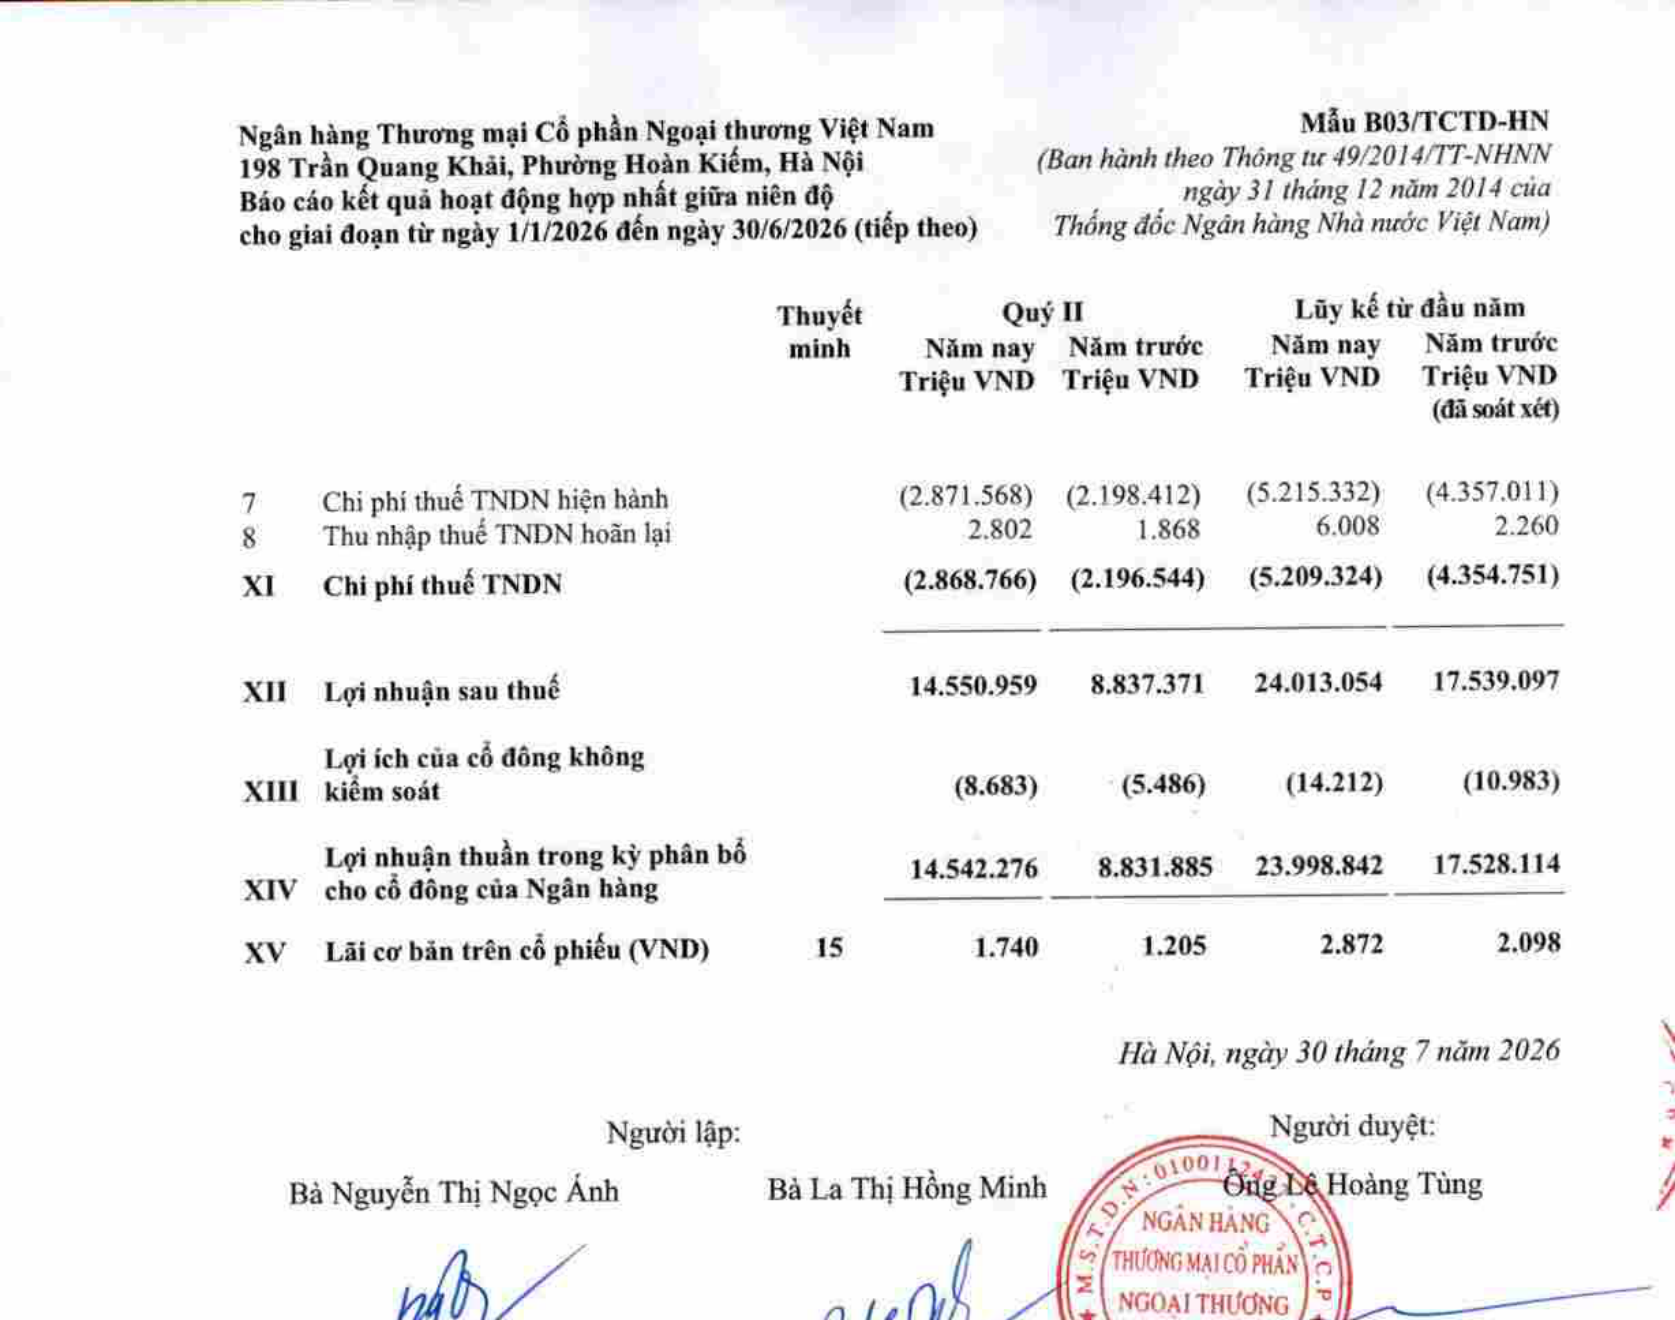
\includegraphics[width=0.8\linewidth]{scan-vcb-kqkd.png}
\caption{Một phần trang KQKD hợp nhất quý 2/2026 của VCB (bản scan, đơn vị triệu đồng). Bốn cột số, mỗi dòng có ký
hiệu La Mã thay vì mã số. Đây là đầu vào điển hình của hệ thống.}\label{fig:scan}
\end{figure}

\section{Nhiều mẫu biểu cùng tồn tại}
Từ năm 2026, Thông tư 99/2025~\cite{tt99} thay Thông tư 200/2014~\cite{tt200} cho doanh nghiệp thường và đánh lại một số
mã. Ngân hàng~\cite{tt49} và công ty chứng khoán~\cite{tt334} có mẫu riêng (Bảng~\ref{tab:mau}).

\begin{table}[H]
\centering\small
\caption{Các mẫu BCTC hệ thống đang hỗ trợ}\label{tab:mau}
\begin{tabularx}{\linewidth}{@{}llX@{}}
\toprule
\textbf{Mẫu} & \textbf{Áp dụng} & \textbf{Điểm cần lưu ý} \\ \midrule
TT200 & DN thường, năm tài chính $\le$ 2025 & Tổng tài sản mã 270 \\
TT99 & DN thường, từ quý 1/2026 & Tổng tài sản đổi sang mã 280; doanh thu, chi phí tài chính dịch từ 21--23 sang
22--24. Khoảng 11\% BCTC quý 2/2026 vẫn in mã 270 \\
TCTD & Ngân hàng & Cấu trúc khác hẳn; nhiều ngân hàng không in mã số mà chỉ có số thứ tự La Mã \\
CTCK & Công ty chứng khoán & Tài sản tài chính FVTPL, cho vay ký quỹ\ldots \\
\bottomrule
\end{tabularx}
\end{table}

Những khó khăn thực tế khi đọc, rút ra từ việc rà khoảng 940 BCTC quý 2/2026:
\begin{itemize}
  \item Khoảng 1/4 BCTC viết \code{1,234,567} thay vì \code{1.234.567}, nên phải suy ra dấu phân cách theo từng tài liệu.
  \item Đơn vị có thể là đồng, nghìn đồng hoặc triệu đồng.
  \item Cột thuyết minh cũng là số nhỏ, dễ nhầm với cột mã số. Cột số thứ tự và cột mã số đôi khi bị đọc đảo cho nhau.
  \item BCTC thật không luôn theo đúng mẫu: có file in mã 270 cho dòng tổng theo mẫu mới, có dòng không in mã, có nhiều
        dòng LCTT trùng mã.
\end{itemize}

\section{Ràng buộc kế toán}
Mỗi BCTC tự chứa nhiều phép cộng, đủ để kiểm tra chéo các con số trong chính nó (Hình~\ref{fig:luoi}). Sai số cho phép
là $\pm 1$ đơn vị làm tròn cho mỗi số hạng.

\begin{figure}[H]
\centering
\begin{tikzpicture}[font=\small\sffamily]
  \node[font=\sffamily\bfseries,color=soigreen] at (3.5,0.95) {BCĐKT};
  \node[gbox=30mm] (ta) at (0,0) {Tổng tài sản\\(270 / 280)};
  \node[gbox=30mm] (tn) at (7,0) {Tổng nguồn vốn\\(440)};
  \draw[very thick,soigreen,<->] (ta) -- node[above,lab]{bằng nhau} (tn);
  \node[box=24mm] (a100) at (-1.7,-1.9) {Tài sản\\ngắn hạn 100};
  \node[box=22mm] (a200) at (1.7,-1.9) {Tài sản\\dài hạn 200};
  \node[box=22mm] (n300) at (5.3,-1.9) {Nợ phải\\trả 300};
  \node[box=22mm] (n400) at (8.7,-1.9) {Vốn chủ\\sở hữu 400};
  \foreach \c in {a100,a200} \draw[arr] (\c) -- (ta);
  \foreach \c in {n300,n400} \draw[arr] (\c) -- (tn);
  \node[box=12mm] (b110) at (-3.4,-3.6) {110};
  \node[box=12mm] (b120) at (-1.7,-3.6) {120};
  \node[box=12mm] (b130) at (0,-3.6) {\ldots};
  \foreach \c in {b110,b120,b130} \draw[arr] (\c) -- (a100);
  \draw[soigray,dashed] (-4.4,-4.5) -- (10.8,-4.5);
  \node[font=\sffamily\bfseries,color=soiamber] at (3.5,-4.95) {KQKD};
  \node[abox=22mm] (i50) at (0,-5.9) {LNTT 50};
  \node[abox=22mm] (i51) at (0,-7.5) {Thuế 51, 52};
  \node[abox=22mm] (i60) at (4.6,-5.9) {LNST 60};
  \node[abox=28mm] (i61) at (9.2,-5.9) {Cổ đông\\công ty mẹ 61};
  \node[abox=28mm] (i62) at (9.2,-7.5) {Cổ đông không\\kiểm soát 62};
  \draw[arr] (i50) -- node[above,lab]{60 = 50 $-$ 51 $-$ 52} (i60);
  \draw[arr] (i51) -| (i60);
  \draw[arr] (i61) -- node[above,lab]{60 = 61 + 62} (i60);
  \draw[arr] (i62) -| ($(i60.south)+(0.5,0)$);
\end{tikzpicture}
\caption{Một phần lưới ràng buộc của BCTC doanh nghiệp thường. Mỗi mũi tên là một phép cộng. Một ô số thường nằm trong
nhiều phép cộng cùng lúc, nên khi đọc nhầm một ô, các phép cộng chứa nó cùng lệch một lượng như nhau.}\label{fig:luoi}
\end{figure}

\begin{table}[H]
\centering\small
\caption{Số mẫu ràng buộc đã khai báo (mỗi mẫu được áp cho từng cột số liệu)}\label{tab:rules}
\begin{tabularx}{\linewidth}{@{}lccX@{}}
\toprule
\textbf{Mẫu} & \textbf{Số ràng buộc} & \textbf{Bắt buộc} & \textbf{Ví dụ} \\ \midrule
TT200 & 41 & 41 & $270 = 100 + 200$, $60 = 50 - 51 - 52$ \\
TT99 & 25 & 13 & $280 = 440$; mã con chưa đối chiếu đủ với phụ lục \\
TCTD & 17 & 16 & thu nhập lãi thuần = thu nhập lãi $-$ chi phí lãi \\
CTCK & 23 & 20 & theo TT334 \\
\bottomrule
\end{tabularx}
\end{table}

Ngoài ràng buộc trong một BCTC, còn có \textbf{ràng buộc giữa các BCTC} của cùng công ty (Hình~\ref{fig:cheoky}).

\begin{figure}[H]
\centering
\begin{tikzpicture}[font=\small\sffamily, scale=0.88, transform shape]
  \foreach \x/\n in {0/Q1,3.3/Q2,6.6/Q3,9.9/Q4} \node[box=17mm] (\n) at (\x,0) {BCTC \n};
  \node[gbox=20mm] (H1) at (3.3,-2.1) {Bán niên\\(soát xét)};
  \node[gbox=20mm] (FY) at (9.9,-2.1) {Năm\\(kiểm toán)};
  \node[box=19mm] (FYp) at (-3.3,0) {Năm trước};
  \draw[arr] (FYp) -- node[above,lab]{đầu năm} (Q1);
  \draw[arr] (Q1) -- node[above,lab]{lũy kế} (Q2);
  \draw[arr] (Q2) -- node[above,lab]{lũy kế} (Q3);
  \draw[arr] (Q3) -- node[above,lab]{lũy kế} (Q4);
  \draw[arr,soigreen,<->] (Q2) -- node[right,lab]{cùng ngày 30/6} (H1);
  \draw[arr,soigreen,<->] (Q4) -- node[right,lab]{cùng ngày 31/12} (FY);
\end{tikzpicture}
\caption{Ràng buộc giữa các kỳ: số đầu năm phải bằng số cuối năm trước; quý = lũy kế kỳ này $-$ lũy kế kỳ trước; BCTC
quý 2 và bán niên (hay quý 4 và năm) cùng ngày nên phải khớp. Khi hai bản khác nhau, đó hoặc là đọc nhầm, hoặc là
doanh nghiệp, kiểm toán đã sửa số.}\label{fig:cheoky}
\end{figure}

\section{Làm sạch số liệu bằng ràng buộc: phương pháp Fellegi--Holt}
Trong thống kê chính thức, số liệu điều tra thường được kiểm tra bằng các quy tắc (edit rules), ví dụ tổng các khoản chi
phải bằng tổng chi. Fellegi và Holt~\cite{fellegi1976} đề xuất nguyên lý: khi một bản ghi vi phạm quy tắc, hãy tìm
\textbf{tập trường nhỏ nhất} cần thay đổi để mọi quy tắc cùng thỏa, thay vì sửa tùy ý từng trường. Bước này gọi là định
vị lỗi (error localization) và là nền của các hệ thống làm sạch số liệu ở cơ quan thống kê~\cite{dewaal2011}.

BCTC có cấu trúc rất giống: các ô số liên kết với nhau bằng phép cộng. Điểm khác là lỗi ở đây chủ yếu do \emph{đọc ảnh}
nhầm 1--2 chữ số, và ta có thể quay lại ảnh gốc để xác nhận. Mục~\ref{sec:loi} trình bày cách Soi tận dụng hai đặc điểm
này.

\section{Mô hình ngôn ngữ đọc ảnh}
Các mô hình ngôn ngữ đa phương thức (VLM) nhận ảnh trang tài liệu và trả về văn bản có cấu trúc, ví dụ JSON theo schema.
So với OCR truyền thống, VLM đọc được bảng nhiều cột, dòng tên bị xuống dòng và chữ tiếng Việt có dấu mà không cần bước
nhận diện vùng bảng riêng. Nhược điểm là đôi khi \enquote{bịa} hoặc đọc nhầm số, và không cho điểm tin cậy cho từng ô.
Vì vậy Soi chỉ dùng VLM để \emph{định vị trang} và \emph{chép nguyên văn}; độ tin cậy đến từ ràng buộc kế toán chứ không
từ mô hình.

\section{Công nghệ sử dụng}
\begin{table}[H]
\centering\small
\caption{Công nghệ sử dụng}\label{tab:congnghe}
\begin{tabularx}{\linewidth}{@{}lX@{}}
\toprule
\textbf{Thành phần} & \textbf{Lựa chọn} \\ \midrule
Ngôn ngữ, web & Python 3.12, FastAPI, Jinja2 (giao diện tạm; trang công khai dự kiến Next.js) \\
CSDL & PostgreSQL 16 + pgvector, migration đánh số \\
Đọc PDF, vẽ ảnh & PyMuPDF \\
Mô hình đọc ảnh & Mô hình thị giác qua API kiểu OpenAI (hiện dùng một mô hình cỡ nhỏ, giá rẻ), đầu ra JSON theo schema \\
Chạy & Docker Compose: \code{db}, \code{web}, \code{watcher}, \code{app} \\
Kiểm thử & pytest, 117 bài kiểm thử; dữ liệu mẫu là tiêu đề và BCTC thật \\
\bottomrule
\end{tabularx}
\end{table}

% ============================================================================
% CHƯƠNG 3: CÁC SẢN PHẨM VÀ NGHIÊN CỨU LIÊN QUAN
% ============================================================================
\chapter{Các sản phẩm và nghiên cứu liên quan}\label{chap:lienquan}

\section{Hệ thống của khóa trước}
Đề tài kế thừa hệ thống \emph{Stock Report Agent} của khóa trước~\cite{prevcohort} (giấy phép MIT). Hệ thống đó dùng
LangGraph gồm các bước hiểu yêu cầu, lấy link BCTC từ Vietstock~\cite{vietstock}, OCR kết hợp Tesseract và Surya
(\enquote{Hybrid OCR}), rồi trích xuất bằng mô hình ngôn ngữ. Trên 401 trang BCTC, Hybrid OCR đạt Number F1 khoảng 85\%,
mỗi báo cáo mất khoảng 5 phút. Bảng~\ref{tab:sosanh} so sánh hai hệ thống.

\begin{table}[H]
\centering\small
\caption{So sánh với hệ thống của khóa trước}\label{tab:sosanh}
\begin{tabularx}{\linewidth}{@{}lXX@{}}
\toprule
& \textbf{Khóa trước} & \textbf{Soi} \\ \midrule
Khi nào đọc & Khi người dùng hỏi (khoảng 5 phút mỗi báo cáo, cần GPU) & Ngay khi BCTC được công bố; người dùng xem
kết quả có sẵn \\
Số cột & Một giá trị cho mỗi chỉ tiêu & Đủ các cột cùng kỳ, lũy kế, đầu năm \\
Đọc số & Hybrid OCR, Number F1 $\approx$ 85\% & Mô hình thị giác chép nguyên văn; code phân tích số \\
Kiểm tra & Không & Ràng buộc kế toán theo mẫu, tự định vị và sửa ô sai \\
Mẫu biểu & Một mẫu & TT200, TT99, TCTD, CTCK \\
Đầu ra & Bảng số trong giao diện chat & Thẻ KQKD, cờ cảnh báo, xếp hạng, lịch, ảnh chia sẻ \\
\bottomrule
\end{tabularx}
\end{table}

\section{Nền tảng dữ liệu tài chính trong nước}
Các cổng thông tin như Vietstock, CafeF cung cấp BCTC dạng PDF, số liệu tổng hợp, biểu đồ và tin tức. Số liệu tổng hợp
thường chỉ có số riêng từng quý, không kèm cột cùng kỳ, lũy kế hay nguồn đến từng trang. Ngày trong kho tài liệu là
ngày đăng lại, không phải giờ công bố chính thức.

\section{Sản phẩm \enquote{AI chứng khoán}}
Nhiều nền tảng đầu tư và công ty chứng khoán đã có trợ lý AI hỏi--đáp, tóm tắt tin tức hay tóm tắt BCTC. Theo thông tin
công khai, các sản phẩm này chủ yếu \emph{bị động} (chờ người dùng hỏi), hiếm khi trích nguồn đến từng ô số, và nhiều
trợ lý gắn với tài khoản của một công ty chứng khoán. Trợ lý AI đa năng tìm được web và đọc được PDF, nhưng không có kho
số liệu đã kiểm chứng để đối chiếu.

\section{Sản phẩm quốc tế}
Ở thị trường quốc tế, Daloopa trích số liệu từ BCTC, mỗi số có link về nguồn; Fiscal.ai và AlphaSense trích dẫn đến
từng câu. Đây là hình mẫu gần nhất của \enquote{lớp số liệu kiểm chứng được} mà Soi hướng tới cho thị trường Việt Nam.

\section{Đánh giá khoảng trống}
\begin{itemize}
  \item Chưa có hệ thống nào cho BCTC Việt Nam dạng scan \emph{tự kiểm chứng} số đọc được bằng ràng buộc kế toán và tự
        sửa lỗi đọc.
  \item Chưa có nguồn miễn phí cung cấp số liệu kèm nguồn đến từng trang, đủ cột so sánh, ghi đúng thời điểm công bố.
  \item Các sản phẩm hiện có ít cảnh báo về chất lượng lợi nhuận: nền thấp, thu nhập bất thường, lãi nhưng dòng tiền âm.
\end{itemize}

% ============================================================================
% CHƯƠNG 4: PHÂN TÍCH, THIẾT KẾ VÀ CÀI ĐẶT
% ============================================================================
\chapter{Phân tích, thiết kế và cài đặt}\label{chap:thietke}

\section{Phân tích yêu cầu}
\subsection{Tác nhân}
\begin{itemize}
  \item \textbf{Khách:} người chưa đăng nhập, chỉ xem được trang chia sẻ thẻ KQKD đã kiểm chứng (ví dụ khi bấm link trên
        Facebook, Zalo).
  \item \textbf{Người dùng được mời:} nhà đầu tư cá nhân đã được mời trong giai đoạn thử nghiệm, đăng nhập bằng link
        gửi qua email.
  \item \textbf{Quản trị viên:} có mọi quyền của người dùng, thêm quyền duyệt tay BCTC và quản lý người dùng.
  \item \textbf{Bộ canh (hệ thống):} tác nhân chạy theo lịch, tự phát hiện BCTC mới, gọi quy trình đọc và gửi email.
\end{itemize}

\subsection{Biểu đồ use case}
\begin{figure}[H]
\centering
\begin{tikzpicture}[font=\small\sffamily]
  \draw[soigray,thick,rounded corners=4pt] (-3.3,-12.4) rectangle (3.3,1.0);
  \node[font=\sffamily\bfseries] at (0,0.6) {Hệ thống Soi};
  % use case: cột giữa
  \node[uc] (u1)  at (0,-0.2)  {Xem trang chia sẻ thẻ};
  \node[uc] (u2)  at (0,-1.2)  {Đăng nhập bằng link email};
  \node[uc] (u3)  at (0,-2.2)  {Xem bảng xếp hạng mùa BCTC};
  \node[uc] (u4)  at (0,-3.2)  {Xem lịch công bố};
  \node[uc] (u5)  at (0,-4.2)  {Xem thẻ KQKD, cờ cảnh báo};
  \node[uc] (u6)  at (0,-5.2)  {Mở trang BCTC gốc của một số};
  \node[uc] (u7)  at (0,-6.2)  {Theo dõi mã, nhận email};
  \node[uc] (u8)  at (0,-7.2)  {Yêu cầu đọc mã ngoài danh sách};
  \node[uc] (u9)  at (0,-8.2)  {Tải BCTC lên};
  \node[uc] (u10) at (0,-9.2)  {Duyệt tay, sửa ô số};
  \node[uc] (u11) at (0,-10.2) {Quản lý người dùng};
  \node[uc] (u12) at (0,-11.4) {Phát hiện, đọc và kiểm chứng\\BCTC mới};
  % tác nhân
  \pic at (-5.4,-0.3) {actor}; \node (kh) at (-5.4,-0.3) {}; \node[below] at (-5.4,-0.8) {Khách};
  \pic at (-5.4,-4.6) {actor}; \node (nd) at (-5.4,-4.6) {}; \node[below,align=center] at (-5.4,-5.1) {Người dùng\\được mời};
  \pic at (5.4,-9.4) {actor}; \node (qt) at (5.4,-9.4) {}; \node[below] at (5.4,-9.9) {Quản trị viên};
  \pic at (5.4,-11.6) {actor}; \node (bc) at (5.4,-11.6) {}; \node[below,align=center] at (5.4,-12.1) {Bộ canh\\(hệ thống)};
  \draw (kh) -- (u1.west);
  \foreach \u in {u2,u3,u4,u5,u6,u7,u8,u9} \draw (nd) -- (\u.west);
  \foreach \u in {u10,u11} \draw (qt) -- (\u.east);
  \draw (bc) -- (u12.east);
  % quản trị viên kế thừa người dùng
  \draw[-{Triangle[open,length=3mm]},thick] (5.4,-8.85) -- (5.4,1.4) -- (-6.3,1.4) -- (-6.3,-4.6) -- (-5.75,-4.6);
  \node[lab,fill=white] at (0,1.4) {quản trị viên có mọi quyền của người dùng};
\end{tikzpicture}
\caption{Biểu đồ use case tổng quát của Soi. Bộ canh phát hiện, đọc, kiểm chứng BCTC mới rồi gửi email cho người theo
dõi mã; yêu cầu đọc mã ngoài danh sách cũng đi qua đúng quy trình này.}\label{fig:usecase}
\end{figure}

\subsection{Yêu cầu chức năng}
\begin{table}[H]
\centering\small
\caption{Các yêu cầu chức năng chính và trạng thái}\label{tab:ycchucnang}
\begin{tabularx}{\linewidth}{@{}lXl@{}}
\toprule
\textbf{Mã} & \textbf{Yêu cầu} & \textbf{Trạng thái} \\ \midrule
F1 & Tự phát hiện BCTC mới của các mã theo dõi, tải về, nhận dạng loại và kỳ & Đã làm \\
F2 & Đọc BCTC (kể cả bản scan), lấy đủ các cột, kiểm chứng bằng ràng buộc kế toán & Đã làm \\
F3 & Tự định vị và sửa ô đọc sai; chuyển duyệt tay khi không tự sửa được & Đã làm \\
F4 & Thẻ KQKD có cờ cảnh báo, mỗi số có nguồn tới trang BCTC & Đã làm \\
F5 & Bảng xếp hạng mùa BCTC, lịch công bố, ảnh thẻ để chia sẻ & Đã làm \\
F6 & Theo dõi mã và nhận email khi có BCTC mới & Đã làm \\
F7 & Yêu cầu đọc mã ngoài danh sách, tải BCTC lên (có hạn mức) & Đã làm \\
F8 & Quản trị: duyệt tay, sửa ô, mời và phân quyền người dùng & Đã làm \\
F9 & Chỉ số tài chính (biên lợi nhuận, ROE\ldots) & Dự kiến \\
F10 & Agent báo cáo so sánh theo câu hỏi của người dùng & Dự kiến \\
\bottomrule
\end{tabularx}
\end{table}

\subsection{Yêu cầu phi chức năng}
\begin{itemize}
  \item \textbf{Đúng số:} chỉ công bố số đã qua ràng buộc bắt buộc hoặc đã được duyệt tay.
  \item \textbf{Truy vết:} mỗi số mở được trang BCTC gốc; mỗi lần sửa được ghi lại người sửa và lý do.
  \item \textbf{Chi phí:} khoảng 0,10 USD mỗi BCTC; có trần chi phí theo ngày và theo tháng (mục~\ref{sec:token}).
  \item \textbf{Độ trễ:} có thẻ trong vài phút sau khi BCTC xuất hiện trên nguồn (sẽ đo trong mùa quý 3/2026).
  \item \textbf{Riêng tư:} tài liệu người dùng tải lên chỉ người đó thấy.
  \item \textbf{Pháp lý:} không đưa khuyến nghị đầu tư; nội dung do AI tạo được gắn nhãn.
\end{itemize}

\section{Kiến trúc tổng thể}
\subsection{Nguyên tắc thiết kế}
\begin{enumerate}
  \item \textbf{Xử lý trước (precompute-first):} tài liệu được xử lý một lần khi công bố, không đợi người dùng hỏi.
  \item \textbf{Số do code tính, chữ do mô hình viết:} mô hình chỉ định vị trang và chép nguyên văn từng ô. Mọi việc
        phân tích số, quy đổi đơn vị và kiểm tra đều do code làm.
  \item \textbf{Không có nguồn thì không nói:} mỗi số mang theo tài liệu, trang và dòng gốc.
  \item \textbf{Kiểm chứng xong mới công bố:} ràng buộc kế toán là cổng chất lượng.
  \item \textbf{Quy tắc khai báo theo mẫu và phiên bản}, không viết cứng trong code.
  \item \textbf{Có phiên bản, không ghi đè:} BCTC công bố lại tạo phiên bản mới; mỗi lần trích xuất ghi phiên bản pipeline.
  \item \textbf{Không khóa vào một nhà cung cấp mô hình:} gọi mô hình qua giao diện kiểu OpenAI.
\end{enumerate}

\subsection{Các thành phần}
\begin{figure}[H]
\centering
\begin{tikzpicture}[font=\small\sffamily]
  \node[box=26mm] (src) at (0,0) {Nguồn công bố\\Vietstock (sau:\\HOSE, HNX)};
  \node[box=26mm] (w) at (3.8,0) {Watcher\\quét định kỳ};
  \node[db] (reg) at (7.6,0) {Kho tài liệu\\(SHA-256)};
  \node[rbox=26mm] (hr) at (3.8,-2.4) {Duyệt tay\\(admin)};
  \node[box=30mm] (pipe) at (7.6,-2.4) {Pipeline đọc\\\& kiểm chứng};
  \node[abox=28mm] (llm) at (12.4,-2.4) {Mô hình thị giác\\(API kiểu OpenAI)};
  \node[box=26mm] (met) at (3.8,-4.8) {Metrics:\\thẻ KQKD, cờ};
  \node[db] (db) at (7.6,-4.8) {PostgreSQL\\số + nguồn};
  \node[gbox=30mm] (web) at (3.8,-7.0) {Web: thẻ, mùa BCTC,\\lịch, ảnh chia sẻ};
  \node[gbox=28mm] (mail) at (7.6,-7.0) {Email khi mã đang\\theo dõi có BCTC};
  \node[circle,draw=soigray,fill=lightgray,minimum size=12mm,font=\small\sffamily] (u) at (5.7,-9.0) {Người dùng};
  \draw[arr] (src) -- (w); \draw[arr] (w) -- (reg); \draw[arr] (reg) -- (pipe);
  \draw[arr,<->] (pipe) -- node[above,lab]{ảnh, JSON} (llm);
  \draw[arr,dashed] (pipe) to[bend right=25] node[above,lab]{còn lệch} (hr);
  \draw[arr,dashed] (hr) to[bend right=25] node[below,lab]{đã sửa} (pipe);
  \draw[arr] (pipe) -- (db);
  \draw[arr] (db) -- (met); \draw[arr] (met) -- (web); \draw[arr] (db) -- (mail);
  \draw[arr] (web) -- (u); \draw[arr] (mail) -- (u);
  \draw[arr,dashed] (u.east) -| node[pos=0.75,right,lab,text width=24mm,align=left]{tải BCTC lên,\\yêu cầu thêm mã} (10.0,-4.0) |- (pipe.south east);
\end{tikzpicture}
\caption{Kiến trúc tổng thể của Soi. Nét liền là luồng chính, nét đứt là luồng phụ (duyệt tay, yêu cầu của người
dùng).}\label{fig:kientruc}
\end{figure}

\subsection{Vòng đời một tài liệu}
\begin{figure}[H]
\centering
\begin{tikzpicture}[font=\small\sffamily]
  \node[box=20mm] (d) at (0,0) {discovered\\(đã thấy)};
  \node[box=20mm] (dl) at (2.8,0) {downloaded\\(đã tải)};
  \node[box=20mm] (ex) at (5.6,0) {extracting\\(đang đọc)};
  \node[gbox=22mm] (v) at (9,1.8) {verified\\(đã kiểm chứng)};
  \node[abox=22mm] (nr) at (9,0) {needs\_review\\(cần duyệt)};
  \node[rbox=22mm] (f) at (9,-1.8) {failed\\(lỗi)};
  \node[gbox=22mm] (ap) at (12.6,0) {approved\\(đã duyệt tay)};
  \draw[arr] (d) -- (dl); \draw[arr] (dl) -- (ex);
  \draw[arr] (ex) -- (v); \draw[arr] (ex) -- (nr); \draw[arr] (ex) -- (f);
  \draw[arr] (nr) -- node[above,lab]{duyệt} (ap);
  \draw[arr,dashed] (nr) -- node[right,lab]{sửa tay} (v);
\end{tikzpicture}
\caption{Trạng thái của một tài liệu. Chỉ \code{verified} và \code{approved} được hiển thị trên thẻ và bảng xếp hạng.
\code{approved} dùng khi phần lệch còn lại là do chính BCTC in lệch, người duyệt ghi rõ lý do.}\label{fig:trangthai}
\end{figure}

\subsection{Luồng xử lý một BCTC mới}
\begin{figure}[H]
\centering
\begin{tikzpicture}[font=\footnotesize\sffamily, scale=0.92, transform shape]
  \foreach \x/\n/\t in {0/w/Bộ canh,2.7/v/Vietstock,5.4/p/Pipeline,8.1/m/Mô hình\\thị giác,10.8/d/CSDL,13.5/u/Người\\theo dõi}{
    \node[life] (\n) at (\x,0) {\t};
    \draw[soigray,dashed] (\n.south) -- (\x,-11.2);
  }
  \newcommand{\msg}[5][msg]{\draw[#1] (#2,#4) -- node[above,font=\scriptsize\sffamily,fill=white,inner sep=1pt]{#5} (#3,#4);}
  \msg{0}{2.7}{-1.0}{lấy danh sách tài liệu}
  \msg[ret]{2.7}{0}{-1.6}{tài liệu mới}
  \msg{0}{2.7}{-2.2}{tải file}
  \msg{0}{5.4}{-2.9}{đọc BCTC}
  \msg{5.4}{8.1}{-3.6}{ảnh nhỏ các trang đầu}
  \msg[ret]{8.1}{5.4}{-4.2}{trang BCĐKT, KQKD, LCTT}
  \msg{5.4}{8.1}{-4.9}{ảnh trang báo cáo}
  \msg[ret]{8.1}{5.4}{-5.5}{bảng chép nguyên văn (JSON)}
  \draw[msg] (5.4,-6.0) -- ++(0.7,0) -- ++(0,-0.5) -- (5.45,-6.5);
  \node[right,font=\scriptsize\sffamily,align=left] at (6.15,-6.25) {chuẩn hóa,\\kiểm tra ràng buộc};
  \draw[soiamber,thick,rounded corners=2pt] (4.4,-6.85) rectangle (9.0,-8.7);
  \node[anchor=north west,font=\scriptsize\sffamily\bfseries,color=soiamber] at (4.45,-6.87) {nếu lệch};
  \msg{5.4}{8.1}{-7.75}{ảnh ô được đề xuất}
  \msg[ret]{8.1}{5.4}{-8.35}{số đọc lại}
  \msg{5.4}{10.8}{-9.3}{lưu số, nguồn, trạng thái}
  \msg[ret]{5.4}{0}{-9.9}{xong}
  \msg{0}{13.5}{-10.6}{email thẻ KQKD (nếu đã kiểm chứng)}
\end{tikzpicture}
\caption{Biểu đồ tuần tự khi một BCTC mới xuất hiện. Mô hình thị giác chỉ được gọi để định vị trang, chép bảng và đọc
lại các ô bị nghi; mọi bước tính toán và kiểm tra đều do code thực hiện.}\label{fig:tuantu}
\end{figure}

\section{Thu thập tài liệu}
\subsection{Lấy danh sách và nhận dạng tiêu đề}
Watcher gọi API danh sách tài liệu của Vietstock (logic kế thừa từ khóa trước) cho các mã đang theo dõi. Từ tiêu đề tiếng
Việt, bộ luật nhận dạng (tệp \code{titles.py} trong module thu thập) xác định bộ khóa: mã, loại báo cáo (quý, bán niên, năm),
kỳ, phạm vi (hợp nhất, riêng, duy nhất), trạng thái soát xét hay kiểm toán, và có phải bản điều chỉnh hay không.
Bộ luật được kiểm thử trên toàn bộ tiêu đề thật của VN30 năm 2025--2026. Lần chạy đầu nhận dạng đúng 174/174 tài liệu.

\subsection{Lưu trữ và phiên bản}
\begin{itemize}
  \item Mỗi file được băm SHA-256. Cùng khóa nhưng khác hash là phiên bản mới, không ghi đè bản cũ.
  \item File nén (\code{.zip}, \code{.rar}) được giải nén và tách thành từng báo cáo.
  \item Lưu thời điểm Vietstock đăng (\code{source\_listed\_at}) và thời điểm hệ thống thấy (\code{discovered\_at}). Giờ
        công bố chính thức (\code{published\_at}) sẽ lấy từ HOSE, HNX ở giai đoạn sau.
\end{itemize}
Kho hiện có 532 tài liệu của 31 mã (VN30 và một mã người dùng yêu cầu thêm), trong đó 120 BCTC đã được đọc. Người dùng
được mời cũng có thể tải lên BCTC riêng; tài liệu tải lên chỉ người đó thấy, không xuất hiện trong dữ liệu công khai.

\section{Đọc và kiểm chứng BCTC}
\subsection{Quy trình}
\begin{figure}[H]
\centering
\begin{tikzpicture}[font=\small\sffamily, node distance=5mm]
  \node[box=58mm] (a) {1. Đánh giá lớp chữ, vẽ ảnh các trang};
  \node[box=58mm, below=of a] (b) {2. Định vị trang BCĐKT, KQKD, LCTT\\(ảnh nhỏ, tối đa 30 trang đầu)};
  \node[box=58mm, below=of b] (c) {3. Chép nguyên văn từng báo cáo\\(STT, mã, tên dòng, thuyết minh, các cột)};
  \node[box=58mm, below=of c] (d) {4. Code chuẩn hóa: dấu phân cách, đơn vị,\\dấu âm, mã số, nhận dạng mẫu};
  \node[abox=58mm, below=of d] (e) {5. Thử các giả thuyết rẻ, không gọi mô hình\\(đảo cột STT/mã, nhãn ngân hàng, mã thiếu)};
  \node[dec, below=7mm of e] (f) {Ràng buộc\\bắt buộc đạt?};
  \node[gbox=30mm, right=14mm of f] (ok) {verified};
  \node[abox=58mm, below=9mm of f] (g) {6. Thang leo thang (mục~\ref{sec:leothang})};
  \node[dec, below=7mm of g] (h) {Đạt?};
  \node[rbox=30mm, right=14mm of h] (nr) {needs\_review\\$\rightarrow$ duyệt tay};
  \node[gbox=30mm, left=14mm of h] (ok2) {verified};
  \draw[arr] (a)--(b); \draw[arr] (b)--(c); \draw[arr] (c)--(d); \draw[arr] (d)--(e); \draw[arr] (e)--(f);
  \draw[arr] (f)-- node[above,lab]{có} (ok); \draw[arr] (f)-- node[right,lab]{không} (g);
  \draw[arr] (g)--(h); \draw[arr] (h)-- node[above,lab]{không} (nr);
  \draw[arr] (h)-- node[above,lab]{có} (ok2);
\end{tikzpicture}
\caption{Quy trình đọc và kiểm chứng một BCTC. Mô hình chỉ tham gia ở bước 2, 3 và các bước đọc lại.}\label{fig:pipeline}
\end{figure}

\subsection{Mô hình chỉ chép, code mới hiểu số}
Mô hình được yêu cầu chép đúng chuỗi in trên trang, ví dụ \code{(2.868.766)}, không tự đổi đơn vị hay tính toán. Đầu ra
là JSON theo schema cố định (Listing~\ref{lst:json}). Code mới là phần phân tích chuỗi thành số:
\begin{itemize}
  \item suy dấu phân cách hàng nghìn của cả tài liệu từ các nhóm 3 chữ số và phép cộng kiểm tra;
  \item đọc đơn vị từ dòng \enquote{Đơn vị tính} và tiêu đề cột;
  \item hiểu số trong ngoặc là số âm;
  \item chuẩn hóa mã số và gán mã chuẩn cho ngân hàng (\code{b.nii}, \code{b.toi}\ldots) theo tên dòng đã bỏ dấu.
\end{itemize}

\begin{center}
\captionof{lstlisting}{Một dòng KQKD sau khi mô hình chép (VCB quý 2/2026)}\label{lst:json}
\begin{Verbatim}[frame=single,fontsize=\small]
{"stt": "XIV", "code": null,
 "label": "Lợi nhuận thuần trong kỳ phân bổ cho cổ đông của Ngân hàng",
 "page": 11,
 "values": {"q_cur": "14.542.276", "q_prev_year": "8.831.885",
            "ytd_cur": "23.998.842", "ytd_prev_year": "17.528.114"}}
\end{Verbatim}
\end{center}

\subsection{Giả thuyết rẻ trước khi gọi lại mô hình}
Nhiều lỗi có dạng lặp lại và sửa được bằng code. Mỗi giả thuyết được \enquote{phân xử} bằng chính các ràng buộc: giữ
phương án làm số ràng buộc đạt nhiều nhất mà không làm mất ràng buộc nào đang đạt.
\begin{itemize}
  \item \textbf{Đảo cột STT và mã số} theo từng trang của từng báo cáo.
  \item \textbf{Nhãn ngân hàng bị xuống dòng:} ghép lại tên dòng rồi so khớp với danh sách nhãn.
  \item \textbf{Mã thiếu:} một dòng không in mã nhưng bằng đúng phần còn thiếu của một ràng buộc thì được gán mã đó.
        Riêng dòng \enquote{LNST của cổ đông công ty mẹ / không kiểm soát} được gán mã 61/62 theo tên dòng (bài học từ
        lỗi VIC, mục~\ref{sec:doichieu}).
  \item \textbf{Ngoại lệ thật của BCTC:} mã 269 (lợi thế thương mại) thuộc tài sản dài hạn khác; nhiều dòng LCTT cùng
        một mã thì cộng lại.
\end{itemize}

\subsection{Thang leo thang khi còn lệch}\label{sec:leothang}
\begin{enumerate}
  \item BCĐKT chưa có đủ tổng tài sản và tổng nguồn vốn thì chép thêm trang kế tiếp, vì có thể bước định vị bỏ sót trang.
  \item \textbf{Tự định vị ô sai bằng ràng buộc, rồi đọc lại riêng các ô đó} (mục~\ref{sec:loi}).
  \item Đọc lại các ô thuộc ràng buộc còn lệch ở độ phân giải cao hơn. Chỉ giữ lần đọc lại nếu số ràng buộc lệch giảm và
        số ràng buộc đạt không giảm.
  \item Chép lại cả báo cáo, mỗi trang một lần gọi, để sửa lỗi bỏ sót dòng; giữ bản ít lệch hơn.
  \item Vẫn lệch thì chuyển duyệt tay. Người duyệt xem ảnh trang cạnh bảng số, sửa từng ô. Mỗi lần sửa được ghi lại và
        trở thành \textbf{dữ liệu vàng} để đánh giá.
\end{enumerate}

\subsection{Bằng chứng cho từng ô}
Sau khi kiểm chứng, mỗi ô số được xếp vào một loại bằng chứng: khớp cả phép cộng lẫn giữa các kỳ; chỉ khớp giữa các kỳ;
chỉ khớp phép cộng; hai BCTC in khác nhau (doanh nghiệp hoặc kiểm toán sửa số); khác kỳ trước do trình bày lại; cần xem
lại; hoặc chưa kiểm được. Giao diện tô màu từng ô theo loại này (Hình~\ref{fig:webtailieu}).

\begin{figure}[H]
\centering
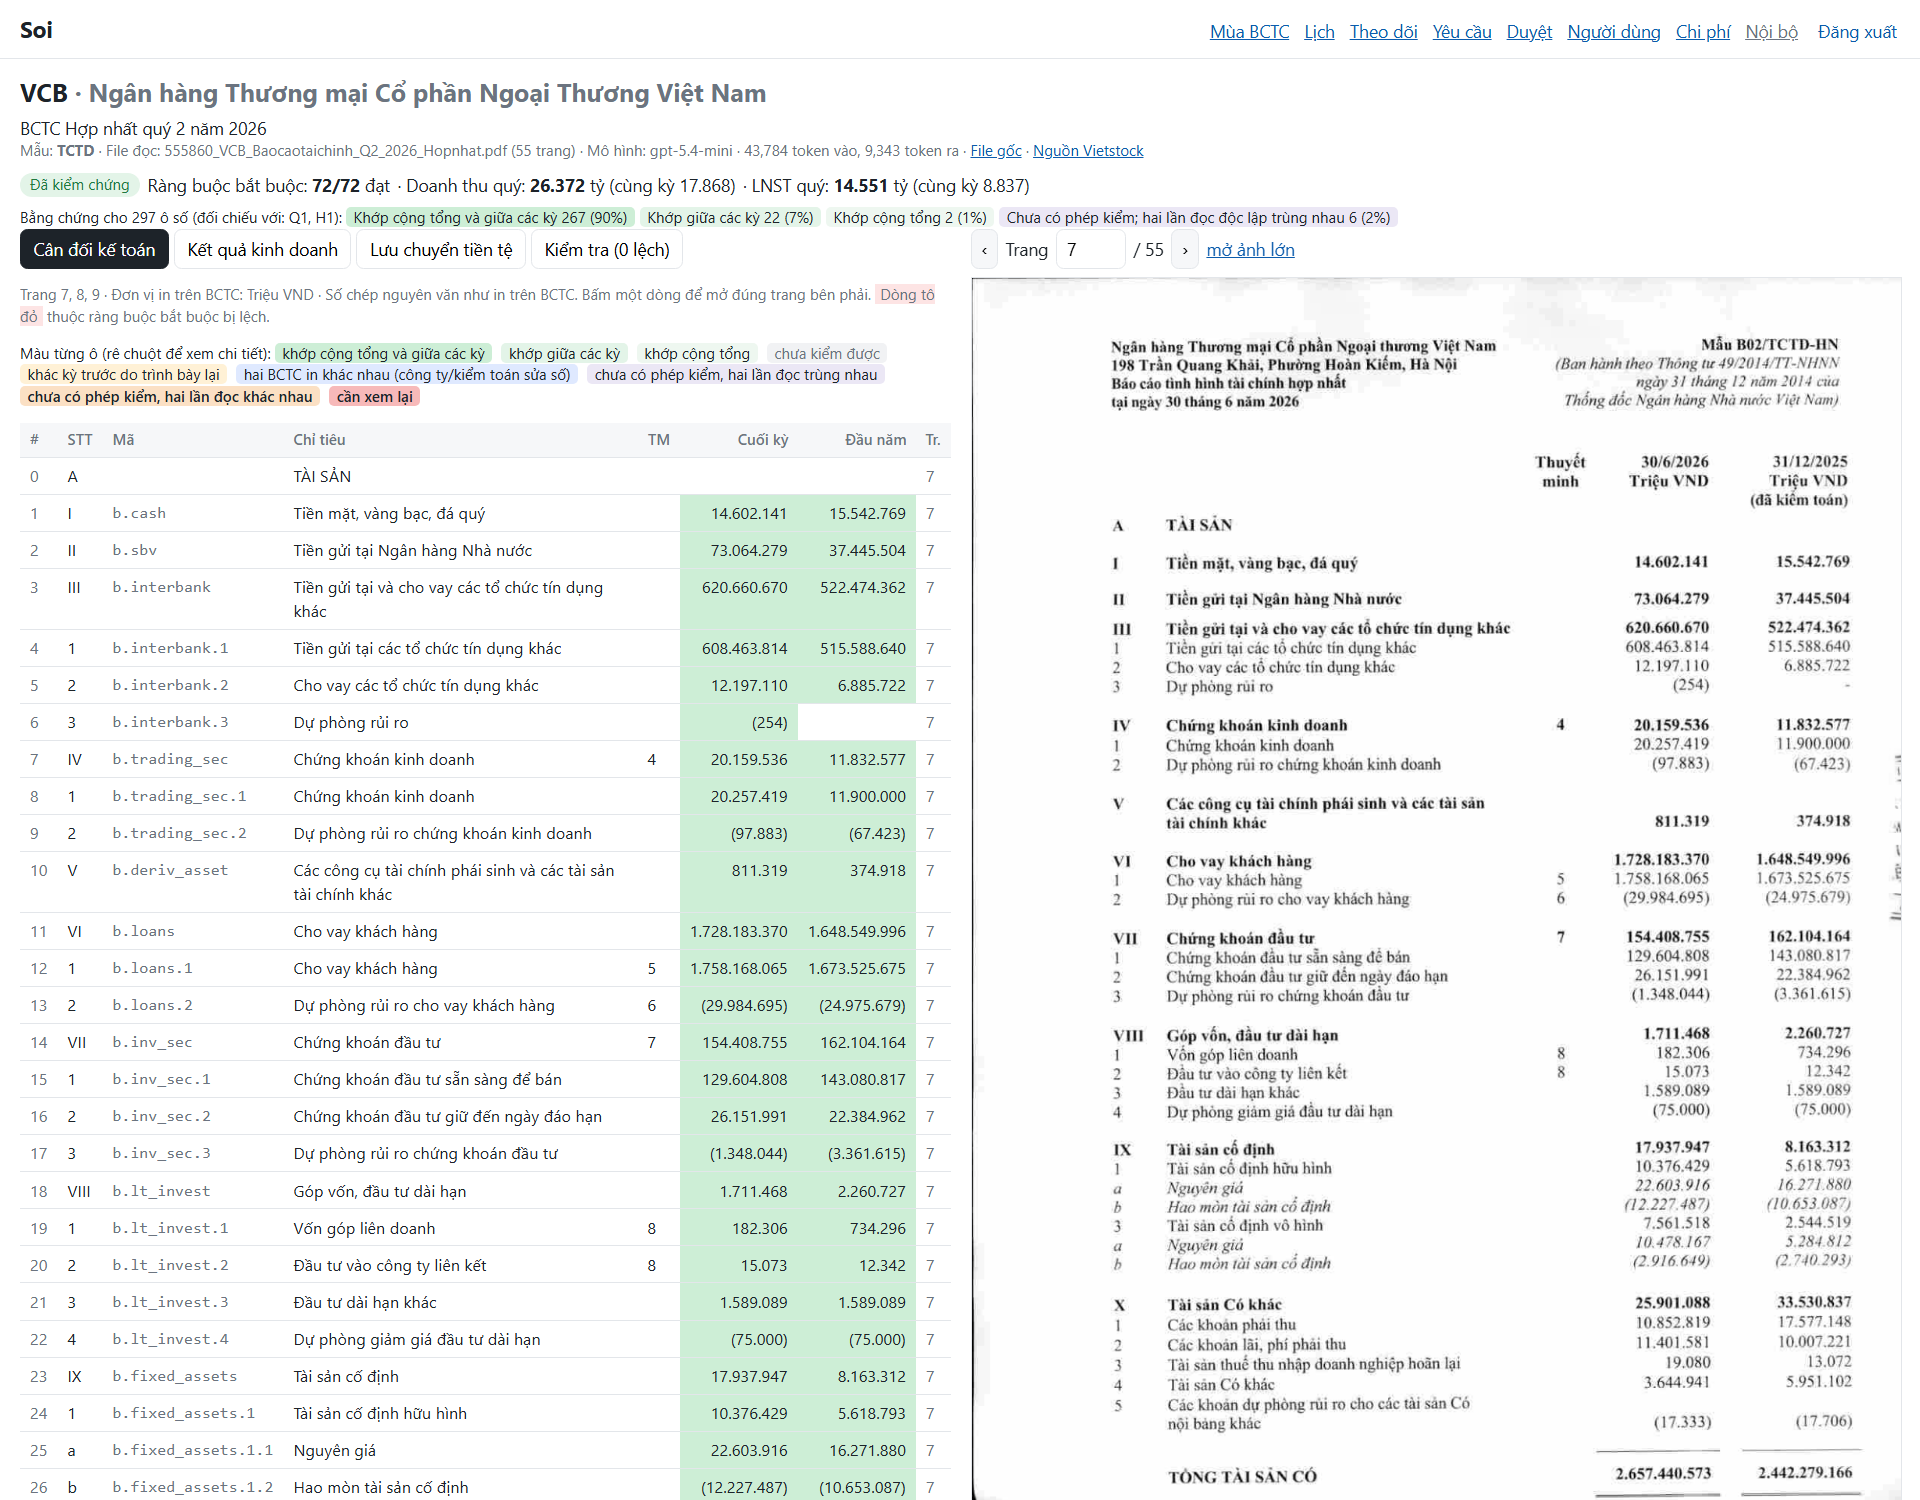
\includegraphics[width=\linewidth]{web-tai-lieu.png}
\caption{Trang tài liệu: bên trái là bảng số đã đọc, tô màu theo bằng chứng; bên phải là ảnh trang BCTC gốc. Bấm một
dòng để mở đúng trang.}\label{fig:webtailieu}
\end{figure}

\section{Công nghệ lõi: tự định vị và tự sửa ô đọc sai}\label{sec:loi}
\subsection{Ý tưởng}
Khi một phép cộng lệch, cách đơn giản là đọc lại \emph{tất cả} các ô trong phép cộng đó. Cách này tốn tiền, và lần đọc
lại cũng có thể sai. Ý tưởng của Soi là \textbf{dùng chính lưới ràng buộc để khoanh vùng ô sai trước}, rồi mới đọc lại,
theo nguyên lý định vị lỗi của Fellegi--Holt~\cite{fellegi1976}. Soi thêm hai điều chỉnh riêng cho lỗi đọc ảnh:
\begin{itemize}
  \item Số đề xuất phải \textbf{giống số cũ về mặt chữ số}: khác nhiều nhất 2 chữ số theo khoảng cách Levenshtein, vì
        đọc nhầm thường chỉ sai 1--2 chữ số. Số đề xuất cũng phải nguyên theo đơn vị in trên BCTC.
  \item Đề xuất \textbf{phải được ảnh xác nhận}: đọc lại riêng ô đó mà không cho mô hình biết con số mong đợi, và chỉ
        nhận khi lần đọc ra đúng số đề xuất. Hai nguồn độc lập là phép cộng và ảnh phải cùng chỉ một con số.
\end{itemize}

\subsection{Thuật toán định vị}
\begin{algorithm}[H]
\caption{Định vị ô đọc sai bằng ràng buộc (rút gọn)}\label{alg:localize}
\begin{algorithmic}[1]
\Require bảng số $S$; tập ràng buộc $R$; tập ràng buộc đang lệch $F \subseteq R$; $\delta_r$ là độ lệch của $r$
\Ensure danh sách đề xuất (ô, số mới, độ tin)
\State $P \gets \emptyset$
\For{ràng buộc $r \in F$, ô $c$ thuộc $r$}
  \State $v \gets$ giá trị làm $r$ khớp nếu thay $c$ \Comment{$v = S[c] \pm \delta_r$}
  \If{$v$ nguyên theo đơn vị in \textbf{và} số chữ số khác với $S[c]$ $\le 2$}
     \State $S' \gets S$ với $S'[c] = v$
     \If{$S'$ làm ít ràng buộc lệch hơn \textbf{và} không làm lệch ràng buộc nào đang đạt}
        \State thêm $(c, v, \text{số ràng buộc được sửa})$ vào $P$
     \EndIf
  \EndIf
\EndFor
\State xét thêm \textbf{cặp ô} cùng lệch một lượng (lỗi lan qua phép cộng giữa chúng)
\State chọn đề xuất sửa được nhiều ràng buộc nhất; nếu nhiều đề xuất ngang nhau và sửa \emph{cùng một tập} ràng buộc
       thì gom thành \textbf{nhóm ngang nhau}
\State áp đề xuất, lặp lại với các ràng buộc còn lệch (tối đa 40 vòng)
\State \Return $P$ kèm độ tin: \emph{cao} (sửa từ 2 ràng buộc trở lên), \emph{vừa}, \emph{thấp}
\end{algorithmic}
\end{algorithm}

\subsection{Xác nhận bằng đọc lại}
\begin{figure}[H]
\centering
\begin{tikzpicture}[font=\small\sffamily, node distance=6mm and 8mm, scale=0.88, transform shape]
  \node[rbox=34mm] (fail) {Ràng buộc lệch\\$100 \ne 110+120+130$};
  \node[box=34mm, right=of fail] (loc) {Định vị: đề xuất\\ô 120 = \textbf{4.83}1 thay vì \textbf{3.83}1};
  \node[box=34mm, right=of loc] (rr) {Đọc lại \emph{riêng} ô 120\\(không đưa số mong đợi)};
  \node[dec, below=9mm of rr] (eq) {Ra đúng\\số đề xuất?};
  \node[gbox=30mm, left=12mm of eq] (acc) {Nhận số mới\\ghi lịch sử sửa};
  \node[dec, below=9mm of eq] (old) {Vẫn ra\\số cũ?};
  \node[abox=34mm, left=12mm of old] (zoom) {Đọc phóng to theo dải\\(4200 px, 3 dải chồng nhau)};
  \node[rbox=30mm, right=10mm of old] (fm) {Nghi BCTC\\tự in lệch};
  \draw[arr] (fail) -- (loc); \draw[arr] (loc) -- (rr); \draw[arr] (rr) -- (eq);
  \draw[arr] (eq) -- node[above,lab]{có} (acc);
  \draw[arr] (eq) -- node[right,lab]{không} (old);
  \draw[arr] (old) -- node[above,lab]{có} (zoom);
  \draw[arr] (zoom) -- node[left,lab]{xác nhận} (acc);
  \draw[arr,dashed] (zoom.south) |- ++(0,-6mm) -| node[pos=0.25,below,lab]{vẫn số cũ} (fm.south);
\end{tikzpicture}
\caption{Đọc lại để xác nhận đề xuất (số trong hình chỉ để minh họa). Với một nhóm đề xuất ngang nhau, hệ thống đọc lại
cả nhóm và chỉ nhận khi đúng \emph{một} ô ra số đề xuất.}\label{fig:xacnhan}
\end{figure}

\begin{ghichu}{Vì sao không đưa con số mong đợi cho mô hình?}
Nếu nói với mô hình \enquote{ô này phải là 4.831}, mô hình có xu hướng đồng ý. Kết quả khi đó không còn là bằng chứng độc
lập. Soi chỉ hỏi \enquote{ô ở dòng X, cột Y ghi số gì}, rồi so câu trả lời với đề xuất bằng code. Phép so bỏ qua khác
biệt về dấu phân cách và dấu ngoặc.
\end{ghichu}

\subsection{Mở rộng sang ràng buộc giữa các BCTC}
Một số lỗi không làm lệch phép cộng nào trong chính BCTC. Ví dụ đọc nhầm một dòng chi tiết không nằm trong ràng buộc bắt
buộc. Khi đó hệ thống dùng thêm các ràng buộc giữa các kỳ (Hình~\ref{fig:cheoky}): số đầu năm bằng số cuối năm trước,
BCTC quý 2 khớp bán niên, quý 4 khớp năm. Nếu hai bản khác nhau, hệ thống đọc lại ô đó trên \emph{cả hai} bản. Số mới
chỉ được nhận khi nó làm hai bản khớp nhau mà không làm lệch ràng buộc bắt buộc nào.

\section{Quản lý token và chi phí}\label{sec:token}
Chi phí gọi mô hình được tính theo số token gửi vào và nhận về:
\begin{equation}
  \text{Chi phí} = p_{\text{vào}} \times N_{\text{vào}} + p_{\text{ra}} \times N_{\text{ra}},
\end{equation}
trong đó $p$ là giá mỗi token theo bảng giá của nhà cung cấp, $N$ là số token. Với mô hình có bước suy luận, token
suy luận được tính vào $N_{\text{ra}}$. Soi giảm cả hai đại lượng bằng các cách sau.

\subsection{Giảm token vào}
\begin{itemize}
  \item \textbf{Chỉ gửi trang cần thiết:} bước định vị dùng ảnh nhỏ (cạnh dài 900 px) của tối đa 30 trang đầu; bước
        chép bảng chỉ gửi đúng các trang BCĐKT, KQKD, LCTT (cạnh dài 2000 px), không gửi cả tài liệu.
  \item \textbf{Đọc lại theo ô:} khi lệch, chỉ hỏi lại vài ô được bước định vị đề xuất, không chép lại cả báo cáo.
        Chép lại cả trang chỉ là bậc sau cùng trước khi chuyển duyệt tay.
  \item \textbf{Giả thuyết rẻ trước:} đảo cột, ghép nhãn, suy mã thiếu đều làm bằng code, không gọi mô hình.
  \item \textbf{Đọc một lần, dùng nhiều lần:} BCTC được đọc một lần khi công bố; file trùng nhận ra bằng SHA-256; ai hỏi
        sau cũng dùng lại kết quả trong kho. Thay đổi quy tắc thì kiểm tra lại trên kết quả đã lưu, không đọc lại ảnh.
\end{itemize}

\subsection{Giới hạn token ra}
Mỗi bước gọi mô hình có trần token ra riêng (Bảng~\ref{tab:tranra}), đặt khoảng 3--4 lần mức lớn nhất đo được, để chặn
trường hợp mô hình trả lời dài bất thường. Đầu ra luôn theo khuôn JSON cố định nên mô hình không viết thêm lời thừa.

\begin{table}[H]
\centering\small
\caption{Trần token ra theo bước và mức đo được (trung bình mỗi lần gọi, lớn nhất trên các BCTC)}\label{tab:tranra}
\begin{tabular}{@{}lrr@{}}
\toprule
\textbf{Bước} & \textbf{Đo được (lớn nhất)} & \textbf{Trần} \\ \midrule
Định vị trang & 1.267 & 6.000 \\
Chép một báo cáo (BCĐKT, KQKD, LCTT) & 5.697 & 24.000 \\
Chép lại một trang & 4.143 & 16.000 \\
Đọc lại ô (kiểm chứng, sửa lỗi, đọc phóng to) & 1.156 & 6.000 \\
Nhận diện file người dùng tải lên & -- & 3.000 \\
\bottomrule
\end{tabular}
\end{table}

\subsection{Đo và giới hạn chi phí}
\begin{itemize}
  \item Mỗi lần gọi được ghi số token vào, ra và thời gian \textbf{theo từng bước}; lệnh \code{cost} in bảng chi phí theo
        bước (Bảng~\ref{tab:chiphi}). Trang tài liệu trên web hiện số token đã dùng cho BCTC đó.
  \item Mỗi người dùng có \textbf{hạn mức yêu cầu mới mỗi ngày}; yêu cầu trả ngay từ kho không tính vào hạn mức.
  \item Tổng chi phí gọi mô hình mỗi tháng không vượt \textbf{trần tháng} (mặc định 5 USD); vượt thì yêu cầu mới nằm chờ
        sang tháng sau, giao diện báo cho người dùng biết.
\end{itemize}

\begin{table}[H]
\centering\small
\caption{Token mỗi báo cáo so với hệ thống của khóa trước}\label{tab:tokenss}
\begin{tabularx}{\linewidth}{@{}p{4.2cm}XX@{}}
\toprule
& \textbf{Khóa trước} & \textbf{Soi} \\ \midrule
Token vào mỗi báo cáo & 272.054 & khoảng 54.000 \\
Token ra mỗi báo cáo & 41.106 & khoảng 13.000 \\
Chi phí mỗi báo cáo & 0,04 USD & khoảng 0,10 USD \\
Ghi chú & Một báo cáo, gửi toàn bộ văn bản OCR cho nhiều bước & Trung bình 120 BCTC, đã gồm mọi lần đọc lại \\
\bottomrule
\end{tabularx}
\end{table}

Soi dùng ít token hơn khoảng 5 lần, nhưng chi phí mỗi báo cáo cao hơn vì mô hình đọc ảnh đắt hơn mô hình khóa trước dùng
cho văn bản OCR, và vì Soi đọc lại để kiểm chứng. Đổi lại, Soi không cần GPU để chạy OCR và mỗi số đều đã được kiểm chứng.

\section{Thẻ KQKD và giao diện}
\subsection{Thẻ KQKD}
Thẻ được tính hoàn toàn bằng code từ số đã kiểm chứng. Mỗi giá trị trên thẻ mang theo nguồn: tài liệu, trang, dòng và
chuỗi gốc. Doanh nghiệp thường có các chỉ tiêu doanh thu thuần, lợi nhuận gộp và LNST của cổ đông công ty mẹ. Ngân hàng
có thu nhập lãi thuần, tổng thu nhập hoạt động, chi phí dự phòng, LNTT và LNST của cổ đông ngân hàng mẹ.

\textbf{Quy tắc hiển thị tăng trưởng:} chỉ in \% khi cả hai kỳ đều lãi. Khi có kỳ lỗ, thẻ mô tả bằng lời, ví dụ
\enquote{lỗ thu hẹp từ 6,8 tỷ còn 3,2 tỷ}, thay vì in \enquote{+53,6\%} gây hiểu nhầm.

\begin{table}[H]
\centering\small
\caption{Các cờ \enquote{cần xem kỹ} trên thẻ. Cờ chỉ nêu số liệu kèm nguồn, không đưa nhận định đầu tư.}\label{tab:co}
\begin{tabularx}{\linewidth}{@{}lX@{}}
\toprule
\textbf{Cờ} & \textbf{Điều kiện (tóm tắt)} \\ \midrule
Lỗ hoặc đổi dấu lợi nhuận & Một trong hai kỳ lỗ: \% không có ý nghĩa \\
Tăng trưởng do nền thấp & Tăng trên 100\% và LNST cùng kỳ dưới 1/3 trung bình 4 quý trước đó \\
Lợi nhuận phần lớn ngoài hoạt động chính & Hơn nửa LNTT không đến từ LN gộp $-$ chi phí bán hàng, quản lý \\
Lợi nhuận tăng nhờ thu nhập khác & Lợi nhuận khác (ngân hàng: lãi thuần hoạt động khác) tăng từ 1/3 mức tăng LNTT và
từ 10\% LNTT quý \\
Hoàn nhập / chi phí dự phòng giảm mạnh & Ngân hàng: dự phòng âm, hoặc giảm quá nửa trong khi LNTT tăng \\
Mua bán công ty con, biến động công ty liên kết & Dòng LCTT về mua, bán công ty con; lãi liên doanh, liên kết tăng
trên 3 lần \\
Có lãi nhưng dòng tiền kinh doanh âm & LNST lũy kế dương, lưu chuyển tiền thuần từ hoạt động kinh doanh âm \\
Số liệu bị sửa giữa các BCTC & Hai BCTC cùng ngày (quý 2 và bán niên\ldots) in khác nhau ở các dòng chính \\
\bottomrule
\end{tabularx}
\end{table}

\begin{figure}[H]
\centering
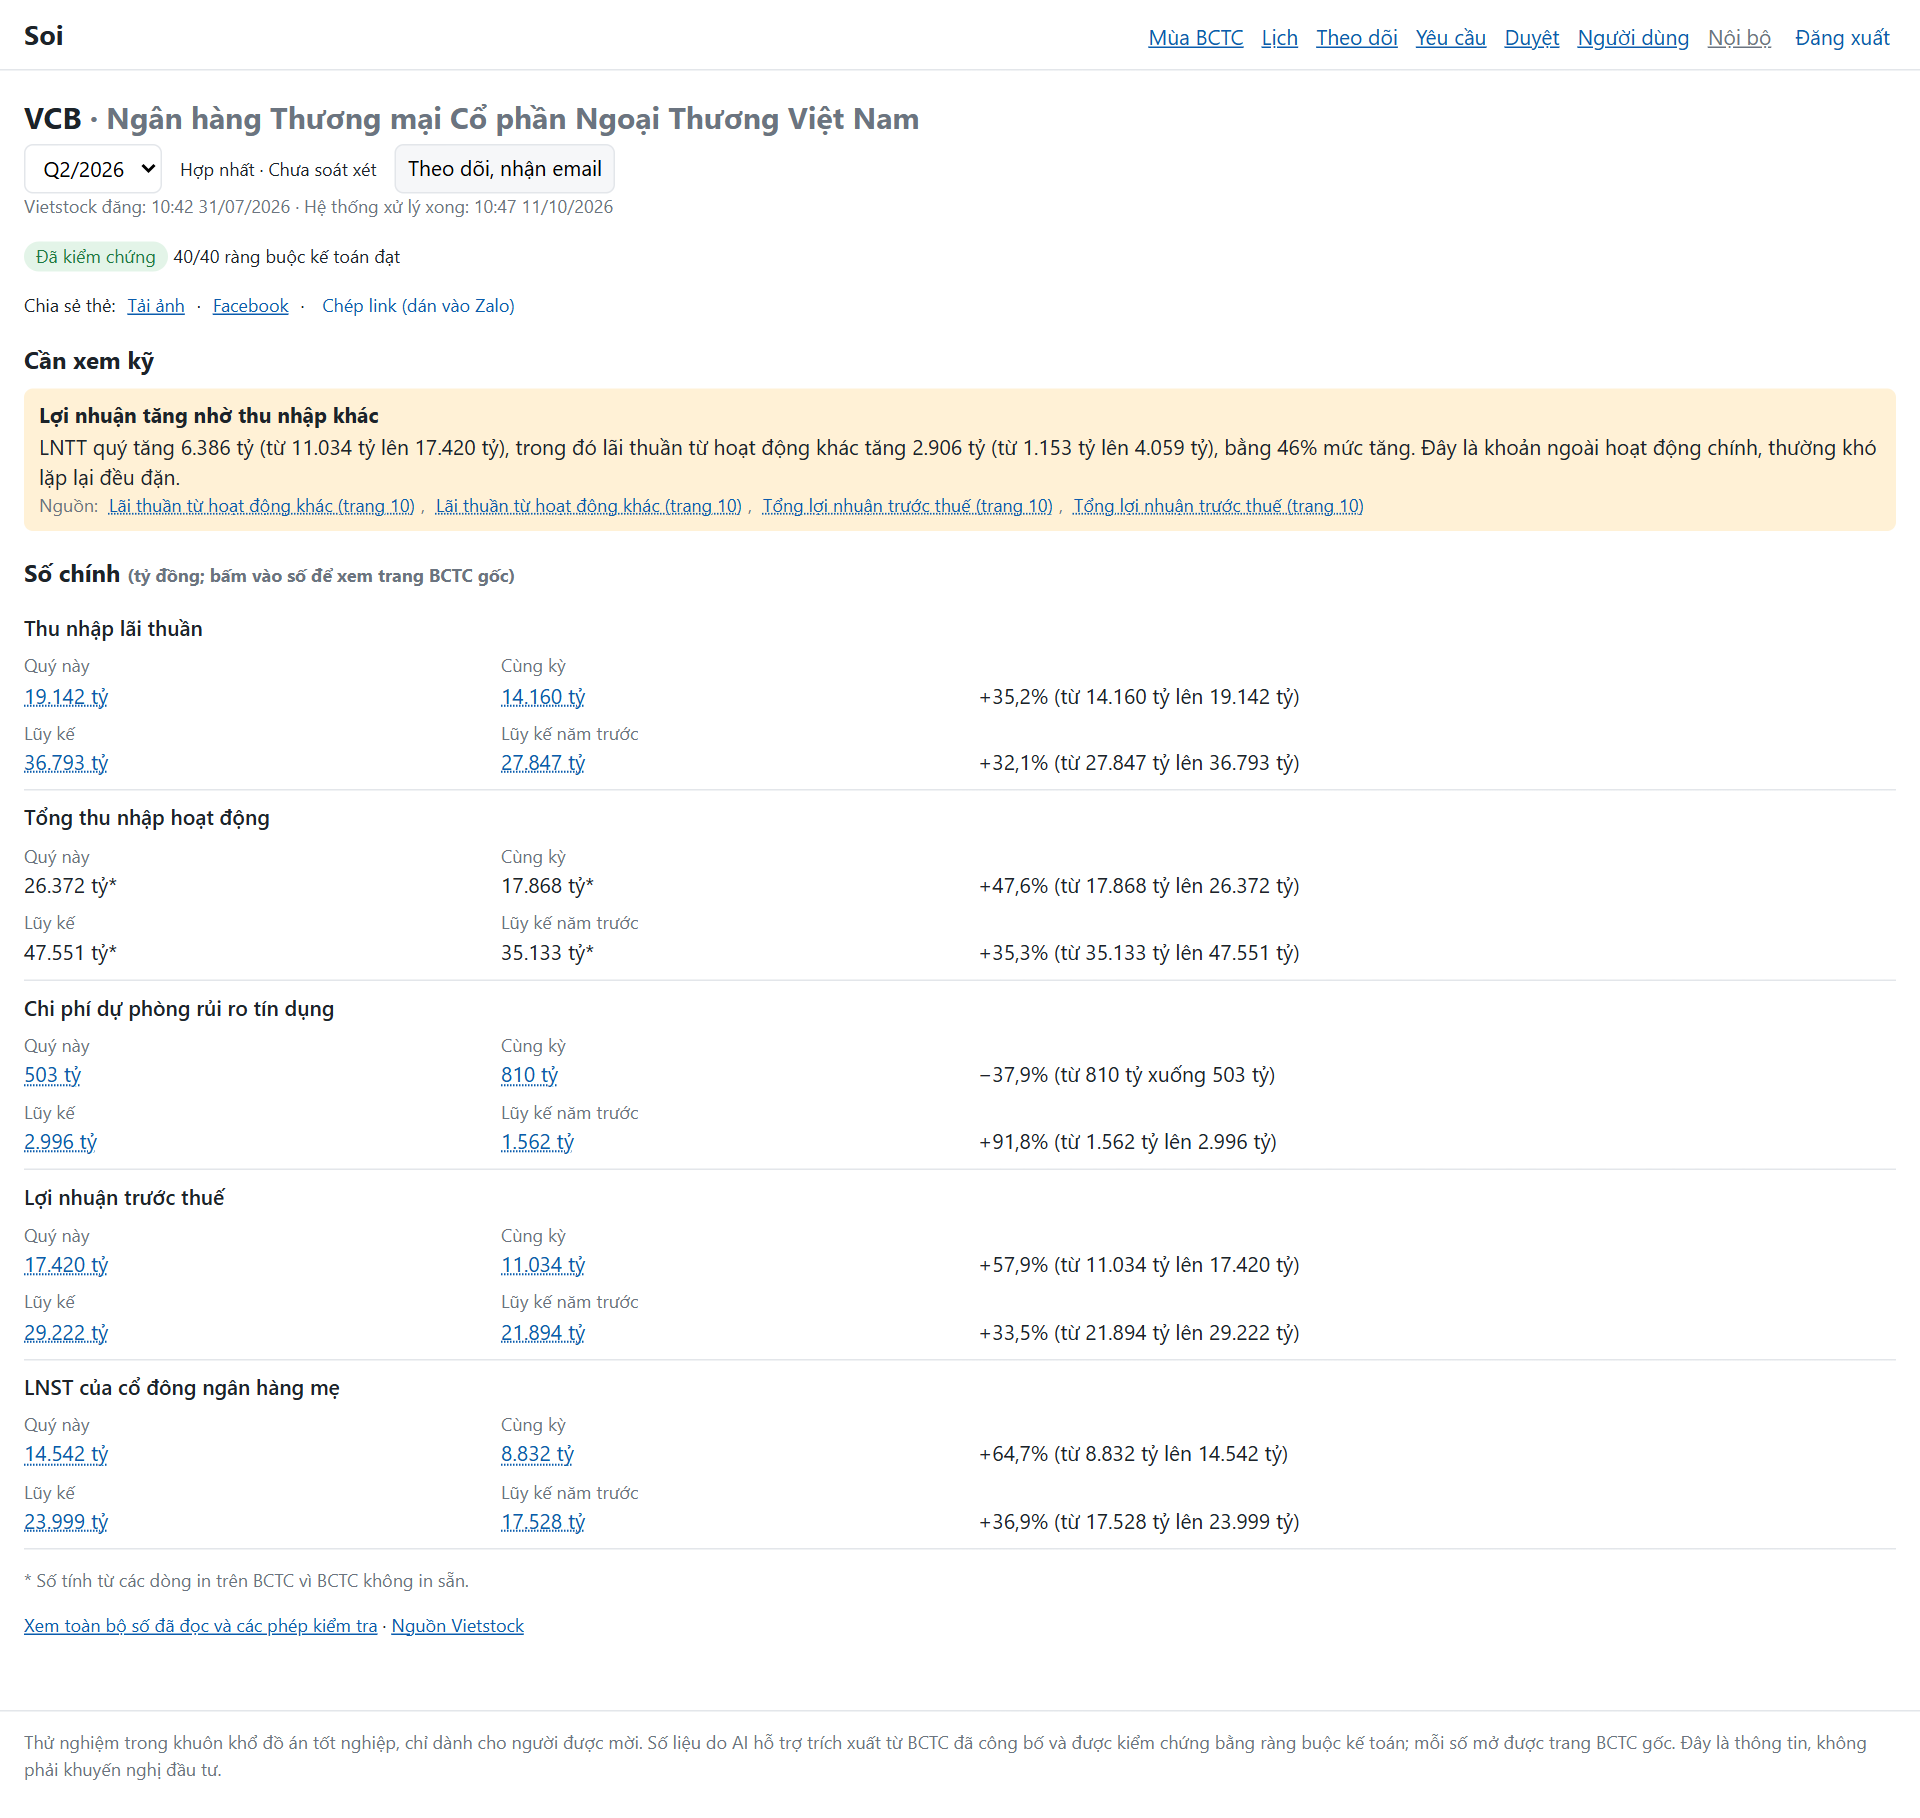
\includegraphics[width=0.9\linewidth]{web-the-vcb.png}
\caption{Thẻ KQKD của VCB quý 2/2026. LNST tăng 64,7\%, và cờ cho thấy gần một nửa mức tăng LNTT đến từ thu nhập hoạt
động khác. Bấm vào mỗi số để mở trang BCTC gốc.}\label{fig:the}
\end{figure}

\subsection{Bảng xếp hạng mùa BCTC}
Bảng xếp hạng các mã theo tăng trưởng LNST quý so với cùng kỳ, chỉ gồm thẻ đã kiểm chứng. Người dùng lọc được theo
loại (ngân hàng, doanh nghiệp), theo \enquote{có cờ} và theo \enquote{số bị sửa} (Hình~\ref{fig:mua}).

\begin{figure}[H]
\centering
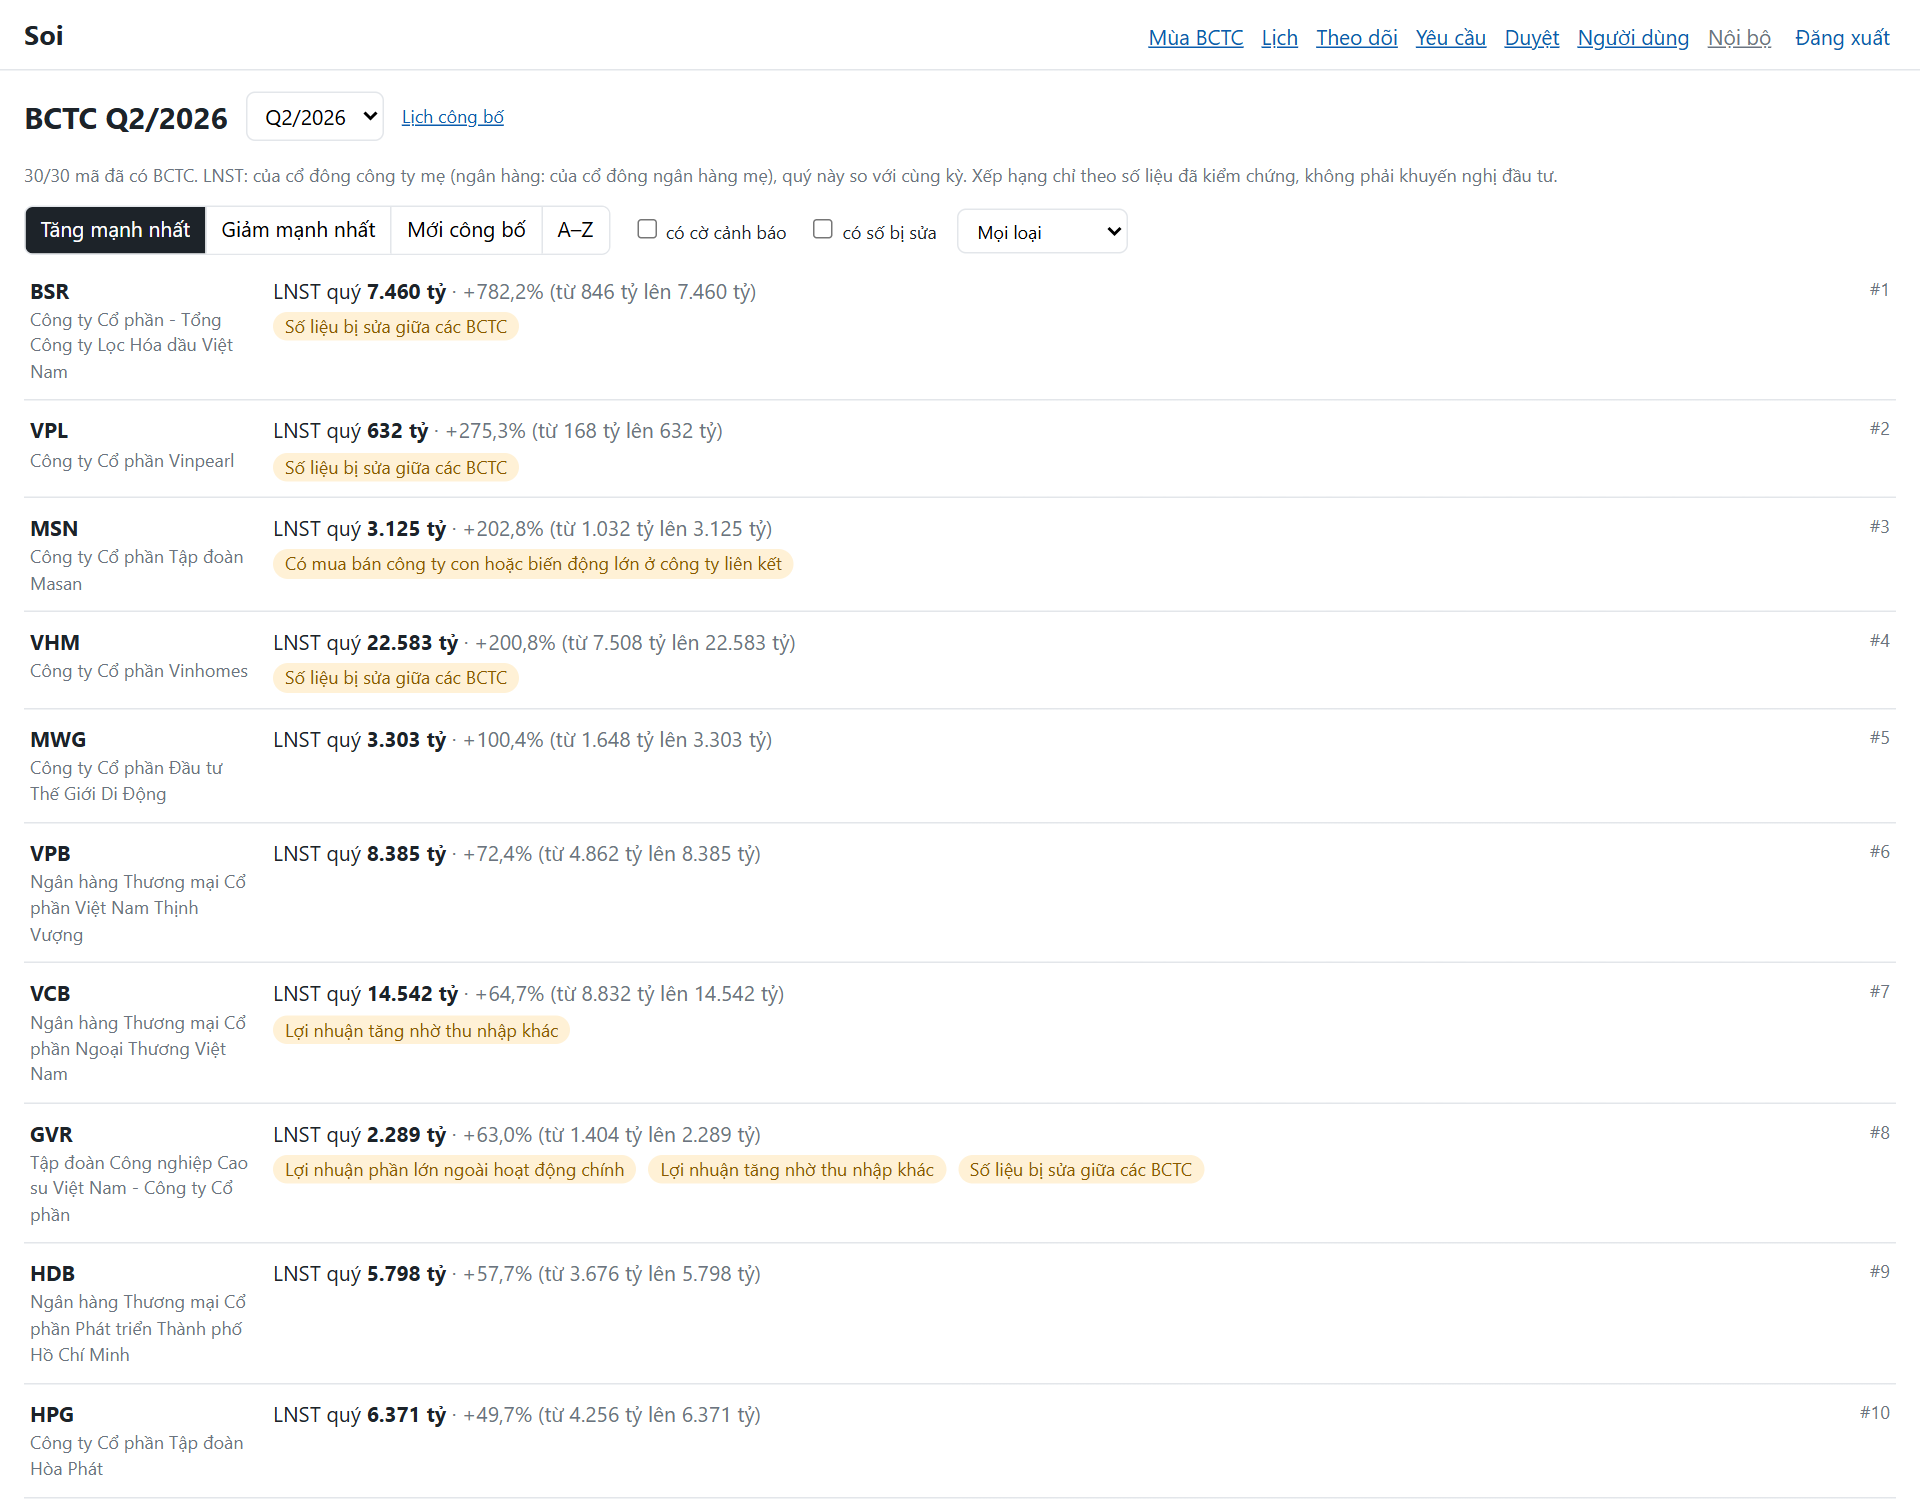
\includegraphics[width=0.95\linewidth]{web-mua-bctc.png}
\caption{Bảng xếp hạng mùa BCTC quý 2/2026 (phần đầu trang).}\label{fig:mua}
\end{figure}

\subsection{Lịch công bố và ảnh chia sẻ}
Lịch công bố cho biết hạn chót của từng mã (20 hoặc 30 ngày sau khi hết quý) và \enquote{ngày dự kiến}. Ngày dự kiến là
trung vị số ngày công bố sau khi hết quý của 8 quý gần nhất. Ảnh thẻ kích thước 1200$\times$630 dùng để chia sẻ lên
Facebook, Zalo; chỉ thẻ đã kiểm chứng mới có trang chia sẻ công khai.

\begin{figure}[H]
\centering
\begin{subfigure}{\linewidth}\centering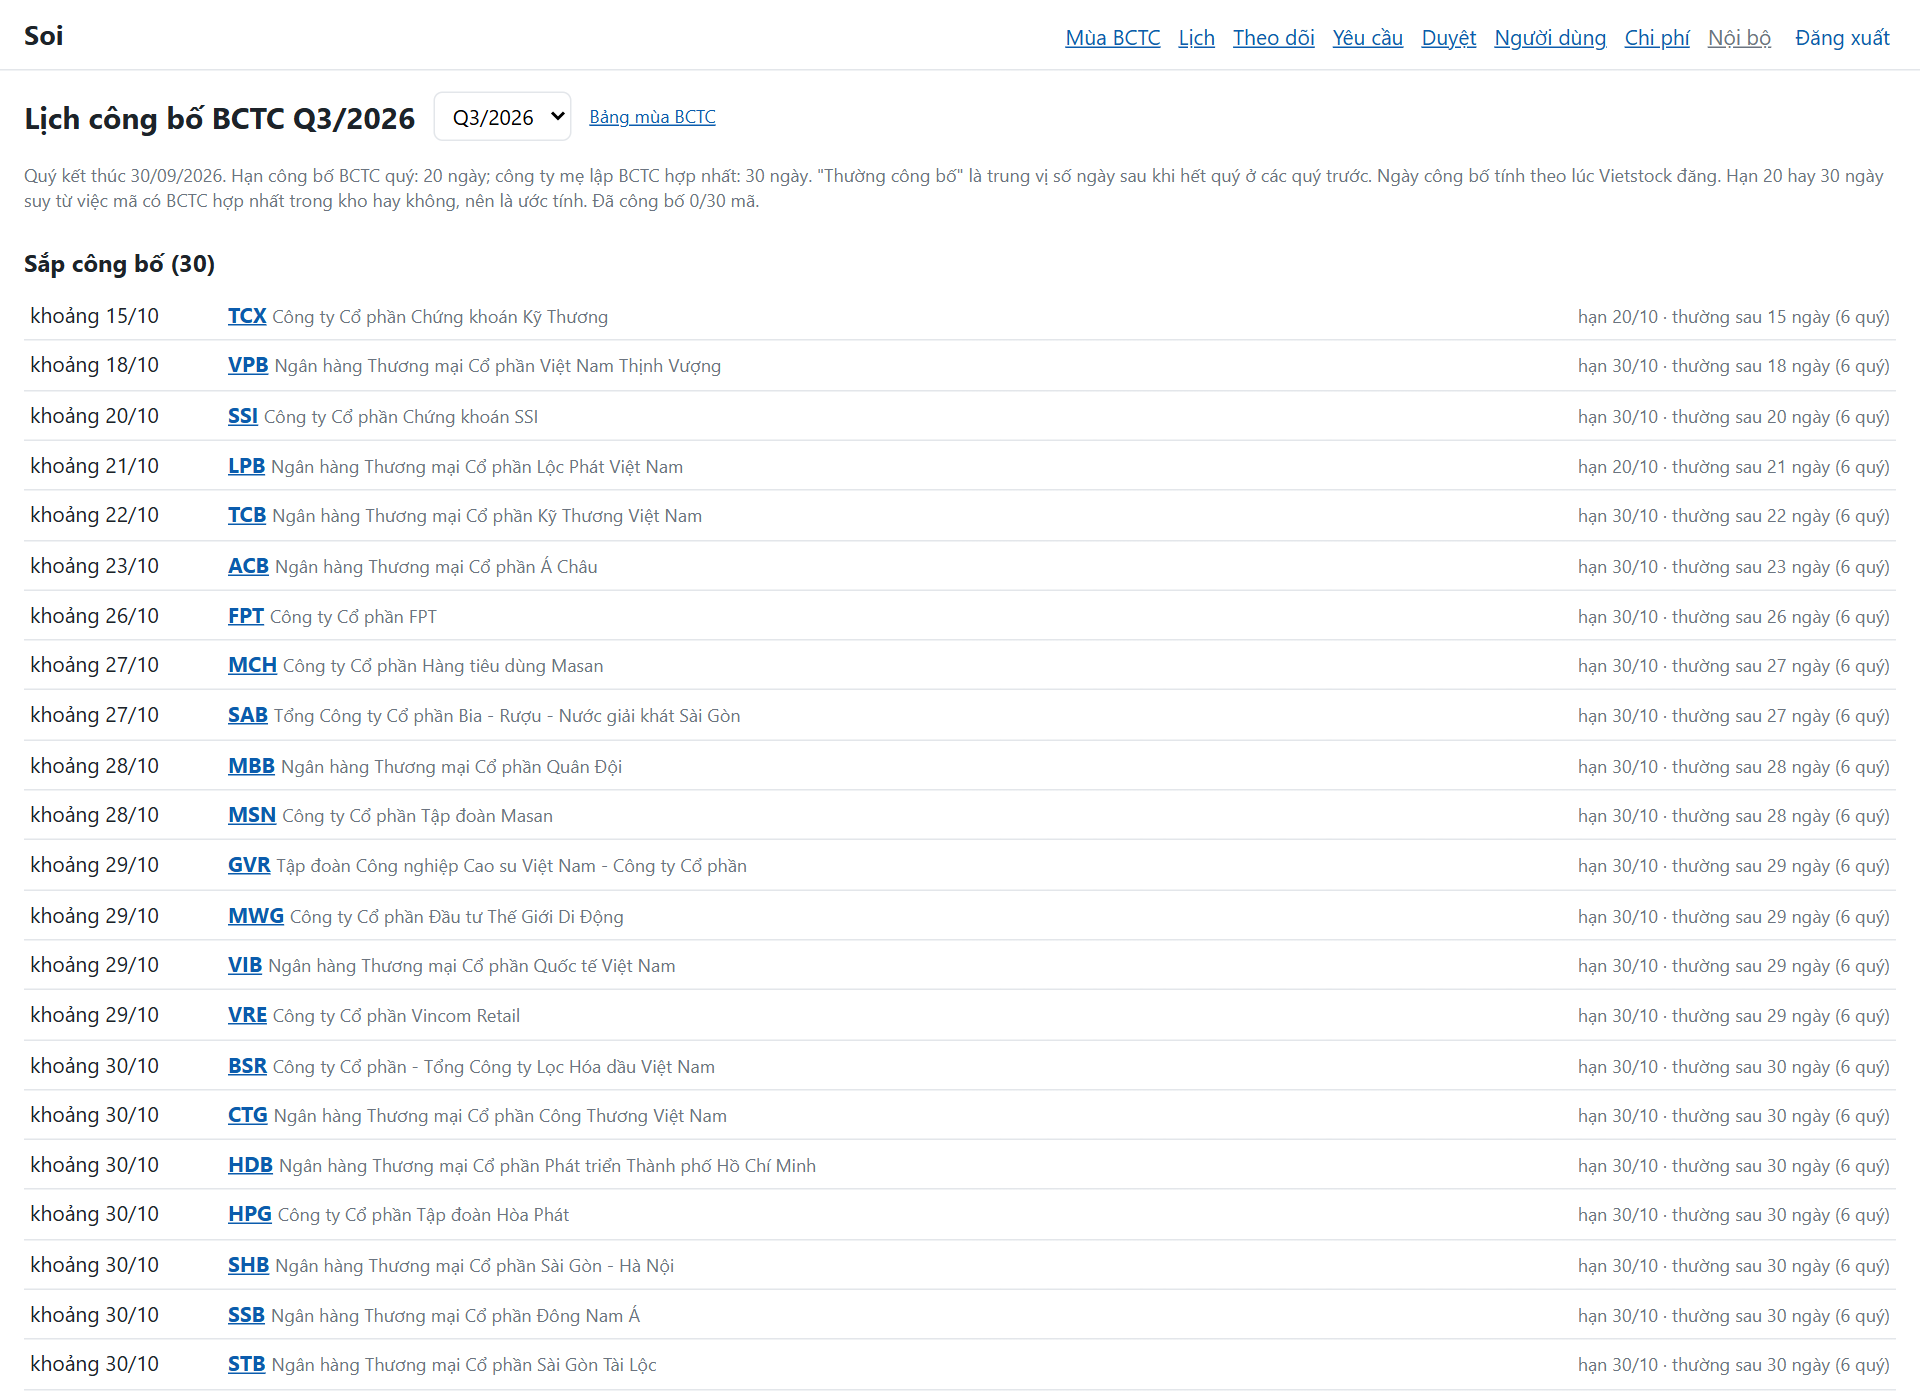
\includegraphics[width=0.95\linewidth]{web-lich.png}\caption{Lịch công bố quý 3/2026 (phần đầu trang)}\end{subfigure}\\[6pt]
\begin{subfigure}{\linewidth}\centering\fbox{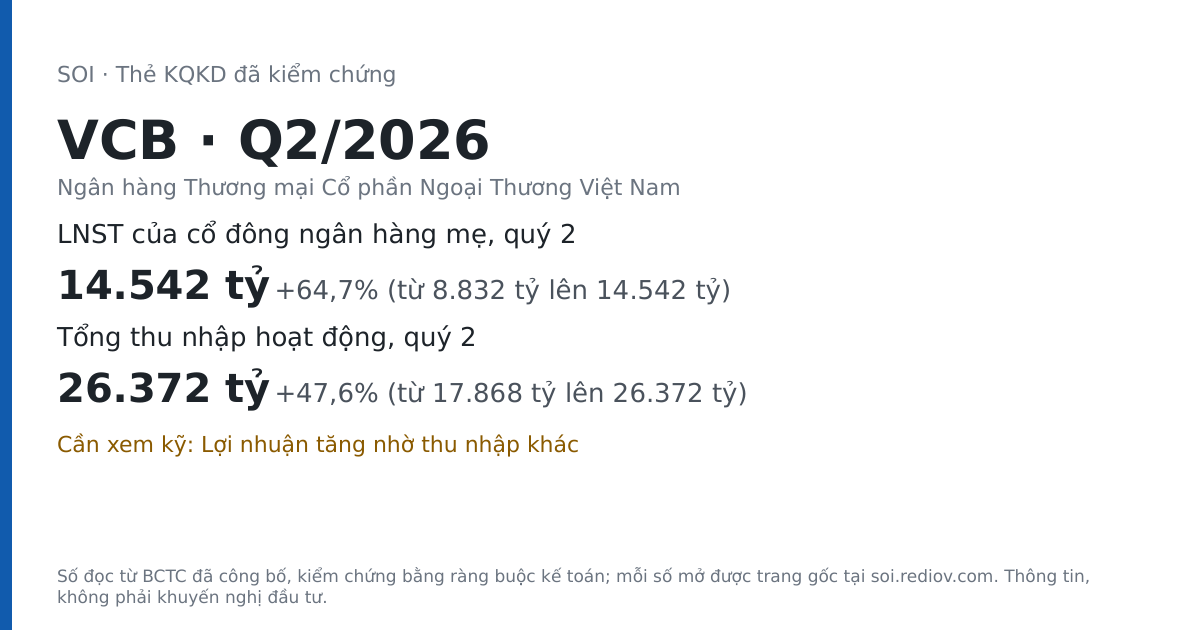
\includegraphics[width=0.62\linewidth]{anh-chia-se-vcb.png}}\caption{Ảnh thẻ để chia sẻ}\end{subfigure}
\caption{Lịch công bố và ảnh thẻ chia sẻ.}\label{fig:lich}
\end{figure}

\subsection{Người dùng và quyền riêng tư}
Giai đoạn thử nghiệm chỉ dành cho người được mời, đăng nhập bằng link gửi qua email. Người dùng theo dõi mã để nhận
email khi có BCTC mới, gửi yêu cầu đọc mã ngoài danh sách (có hạn mức mỗi ngày), hoặc tải lên BCTC riêng. Tài liệu tải
lên chỉ chủ sở hữu thấy.

% ============================================================================
% CHƯƠNG 5: KẾT QUẢ THỰC NGHIỆM VÀ ĐÁNH GIÁ
% ============================================================================
\chapter{Kết quả thực nghiệm và đánh giá}\label{chap:danhgia}

\section{Tỷ lệ BCTC đạt kiểm chứng}
\begin{figure}[H]
\centering
\begin{tikzpicture}
\begin{axis}[ybar stacked, bar width=14mm, width=0.86\linewidth, height=6.4cm,
  symbolic x coords={Q4/2025,Q1/2026,Q2/2026,H1/2026}, xtick=data,
  ylabel={Số BCTC}, ymin=0, ymax=36, enlarge x limits=0.18,
  legend style={at={(0.5,-0.18)},anchor=north,legend columns=4,font=\small},
  nodes near coords, nodes near coords style={font=\scriptsize},
  tick label style={font=\small}, label style={font=\small}]
\addplot[fill=soigreen!75,draw=soigreen] coordinates {(Q4/2025,25) (Q1/2026,30) (Q2/2026,31) (H1/2026,21)};
\addplot[fill=soiblue!55,draw=soiblue] coordinates {(Q4/2025,4) (Q1/2026,0) (Q2/2026,0) (H1/2026,0)};
\addplot[fill=soiamber!70,draw=soiamber] coordinates {(Q4/2025,0) (Q1/2026,0) (Q2/2026,0) (H1/2026,9)};
\addplot[fill=soired!70,draw=soired] coordinates {(Q4/2025,1) (Q1/2026,0) (Q2/2026,0) (H1/2026,0)};
\legend{Đã kiểm chứng, Đã duyệt tay, Cần duyệt, Lỗi}
\end{axis}
\end{tikzpicture}
\caption{Trạng thái 120 BCTC đã đọc (VN30, cộng một mã ngoài VN30 do người dùng yêu cầu ở quý 2/2026). BCTC quý: 90/91
đạt kiểm chứng hoặc được duyệt tay. BCTC bán niên có 9 bản còn chờ duyệt.}\label{fig:trangthaiketqua}
\end{figure}

Bốn BCTC quý 4/2025 \enquote{đã duyệt tay} (BSR, SSB, VPL, VHM) là trường hợp chính BCTC tự cộng lệch. Lần đọc lại phóng
to vẫn ra đúng số cũ, nên người duyệt ghi rõ lý do rồi duyệt. Bản lỗi duy nhất (TCX quý 4/2025) là một công ty chứng khoán
có cấu trúc trang khác thường.

\section{Chi phí}
\begin{table}[H]
\centering\small
\caption{Chi phí gọi mô hình cho 120 BCTC (tổng khoảng 11,98 USD, tức khoảng 0,10 USD mỗi BCTC)}\label{tab:chiphi}
\begin{tabular}{@{}lrr@{}}
\toprule
\textbf{Bước} & \textbf{Số lần gọi} & \textbf{USD} \\ \midrule
Định vị trang & 36 & 0,64 \\
Chép BCĐKT, KQKD, LCTT (lần đầu, đã ghi theo bước) & 90 & 1,79 \\
Chép lại báo cáo còn lệch & 78 & 0,97 \\
Đọc lại ô (kiểm chứng chéo kỳ, ô lệch) & 79 & 0,28 \\
Các lần chạy trước khi ghi chi phí theo bước & 474 & 8,32 \\ \midrule
\textbf{Tổng} & \textbf{757} & \textbf{11,98} \\
\bottomrule
\end{tabular}
\end{table}

\section{Định vị ô đọc sai}\label{sec:evalrepair}
Bộ đánh giá \code{eval/repair.py} không gọi mô hình. Nó lấy các ô \emph{đã biết là đọc sai}: các ô được sửa tay, và các
ô đọc lại thành công ở BCTC nay đã kiểm chứng. Bộ đánh giá trả các ô đó về số sai ban đầu, chạy bước định vị, rồi so
đề xuất với số đúng. Bộ đề gồm 41 ô thuộc 16 BCTC. 7 ô \enquote{ngoài tầm}: không ràng buộc nào, trong BCTC hay giữa các
kỳ, chỉ ra chúng. Kết quả trên 34 ô còn lại ở Hình~\ref{fig:evalrepair}.

\begin{figure}[H]
\centering
\begin{tikzpicture}
\begin{axis}[xbar, bar width=7mm, width=0.8\linewidth, height=5.2cm, xmin=0, xmax=20,
  symbolic y coords={Sót,Cần đọc lại cả nhóm,Đúng ô đúng số}, ytick=data,
  xlabel={Số ô (trên 34 ô trong tầm)}, nodes near coords, nodes near coords align={horizontal},
  tick label style={font=\small}, label style={font=\small}, enlarge y limits=0.3]
\addplot[fill=soiblue!60,draw=soiblue] coordinates {(9,Đúng ô đúng số) (15,Cần đọc lại cả nhóm) (10,Sót)};
\end{axis}
\end{tikzpicture}
\caption{Kết quả định vị. \enquote{Đúng}: một đề xuất duy nhất, đúng ô, đúng số. \enquote{Cần đọc lại}: ô sai nằm trong
một nhóm đề xuất ngang nhau có phương án đúng; đọc lại cả nhóm sẽ chọn ra (15 nhóm, tổng 52 ô phải đọc lại, 3 trường
hợp nhờ đối chiếu kỳ khác). \enquote{Sót}: không có đề xuất, phần lớn là nhiều lỗi chồng lên nhau trong một cột.
Có 2 đề xuất sai, cả hai đều bị bước đọc lại loại.}\label{fig:evalrepair}
\end{figure}

Trong các lần chạy thật, mọi số được bước \enquote{định vị $\rightarrow$ đọc lại xác nhận} chấp nhận đều đúng khi đối
chiếu với ảnh gốc. Ví dụ BCTC bán niên HDB: một ô BCĐKT đọc sai được sửa đúng nhờ đề xuất của bước định vị. Bước đọc
phóng to theo dải sửa được một ô VHM mà lần đọc lại thường vẫn nhầm.

\section{Đối chiếu với nguồn dữ liệu công khai}\label{sec:doichieu}
Sau mỗi mùa BCTC, lệnh \code{eval/external.py} so các chỉ tiêu trên thẻ với bảng KQKD theo quý của một trang dữ liệu
tài chính công khai. Số của nguồn ngoài \textbf{chỉ dùng nội bộ}, không hiển thị trên Soi.

\begin{figure}[H]
\centering
\begin{tikzpicture}
\begin{axis}[xbar stacked, bar width=6mm, width=0.66\linewidth, height=5.6cm, xmin=0, xmax=90,
  symbolic y coords={Tổng thu nhập HĐ ngân hàng,LNST công ty mẹ,Lợi nhuận gộp,Doanh thu thuần}, ytick=data,
  xlabel={Số ô (VN30, quý 4/2025, 1/2026, 2/2026)},
  legend style={at={(0.5,-0.28)},anchor=north,legend columns=2,font=\small},
  tick label style={font=\small}, label style={font=\small}, enlarge y limits=0.2]
\addplot[fill=soigreen!70,draw=soigreen] coordinates {(45,Doanh thu thuần) (44,Lợi nhuận gộp) (81,LNST công ty mẹ) (38,Tổng thu nhập HĐ ngân hàng)};
\addplot[fill=soiamber!80,draw=soiamber] coordinates {(0,Doanh thu thuần) (1,Lợi nhuận gộp) (2,LNST công ty mẹ) (0,Tổng thu nhập HĐ ngân hàng)};
\legend{Khớp, Lệch (số của Soi khớp phép cộng của chính BCTC)}
\end{axis}
\end{tikzpicture}
\caption{Đối chiếu với nguồn ngoài: 208/211 ô khớp. 3 ô lệch (VJC quý 1/2026 chênh 2 nghìn đồng; VHM quý 4/2025 chênh
200 triệu đồng) đều là trường hợp số của Soi thỏa ràng buộc của chính BCTC.}\label{fig:doichieu}
\end{figure}

\begin{ghichu}{Bài học: lỗi \enquote{đọc đúng số nhưng lấy nhầm dòng}}
Lần đối chiếu đầu tìm ra một lỗi thật của Soi. BCTC quý 1/2026 của VIC không in mã cho hai dòng \enquote{LNST của cổ
đông công ty mẹ} và \enquote{của cổ đông không kiểm soát}. Thẻ không tìm thấy dòng công ty mẹ nên lấy dòng LNST tổng.
Kết quả thẻ hiện LNST công ty mẹ 5.611 tỷ, \textbf{tăng khoảng 150\%}, trong khi số đúng là 7.276 tỷ, \textbf{tăng
4,3\%}. Mọi ô đều được đọc đúng, nên bộ kiểm chứng không bắt được lỗi này.

Cách sửa: gán mã 61/62 theo tên dòng khi BCTC không in mã. Nhờ đó ràng buộc $61 + 62 = 60$ kiểm được hai dòng này.
Rút ra: ràng buộc kế toán bắt được lỗi \emph{đọc sai số}, nhưng cần thêm đối chiếu nguồn ngoài để bắt lỗi \emph{lấy
nhầm dòng}. Vì vậy đối chiếu nguồn ngoài đã trở thành bước cố định sau mỗi mùa BCTC.
\end{ghichu}

\section{Tốc độ và các thước đo khác}
\chualam
\begin{itemize}
  \item Time-to-Insight: từ lúc BCTC xuất hiện tới lúc thẻ được công bố, p50/p95, đo trong mùa quý 3/2026.
  \item Độ chính xác theo ô trên bộ dữ liệu vàng (50--100 BCTC duyệt tay).
  \item So sánh Number F1 với baseline của khóa trước trên bộ vnpdf.
\end{itemize}

% ============================================================================
% CHƯƠNG 6: KẾT LUẬN VÀ HƯỚNG PHÁT TRIỂN
% ============================================================================
\chapter{Kết luận và hướng phát triển}\label{chap:ketluan}

\section{Kết luận}
Đến giữa tháng 10/2026, Soi đã có đủ chuỗi xử lý: thu thập BCTC, đọc bằng mô hình thị giác, kiểm chứng bằng ràng buộc kế
toán, tự định vị và sửa ô đọc sai, tính thẻ KQKD có cờ cảnh báo, và giao diện web. Trên VN30, gần như toàn bộ BCTC quý đạt
kiểm chứng với chi phí khoảng 0,10 USD mỗi BCTC. Đối chiếu với nguồn ngoài cho thấy số liệu khớp ở 208/211 ô, và cả 3 ô
lệch đều có lời giải thích từ chính BCTC.

Điểm khác biệt của hệ thống không nằm ở mô hình ngôn ngữ, vì ai cũng dùng được mô hình như nhau. Điểm khác biệt là
\textbf{lớp kiểm chứng}: mỗi con số đều có nguồn, đều đã qua kiểm tra, và có lịch sử sửa lỗi tích lũy qua từng mùa. Các
giai đoạn tiếp theo sẽ đặt agent phân tích lên trên lớp số liệu này.

\section{Hướng phát triển}
Các mục dưới đây đã có trong kế hoạch nhưng chưa thực hiện. Mỗi mục sẽ được viết đầy đủ khi hoàn thành.

\subsection{Chạy thật mùa BCTC quý 3/2026 cho VN30}\chualam
\subsection{Chỉ số tài chính: biên lợi nhuận gộp, ROE, tăng trưởng lũy kế}\chualam
\subsection{Agent báo cáo so sánh (lập kế hoạch, gọi công cụ, kiểm tra số khi viết)}\chualam
\subsection{Bộ kiểm tra số và từ chỉ hướng trong văn bản sinh ra}\chualam
\subsection{Bộ dữ liệu vàng và benchmark vnpdf}\chualam
\subsection{Phép thử so với trợ lý AI đa năng}\chualam
\subsection{Mở rộng lên VN100}\chualam
\subsection{Tìm nguyên nhân biến động trong thuyết minh và công văn giải trình}\chualam
\subsection{Sàng lọc doanh nghiệp tăng trưởng và kiểm định lịch sử (backtest)}\chualam
\subsection{Radar sự kiện công bố thông tin và bản tin sáng theo danh mục}\chualam
\subsection{Kênh phân phối: Facebook, Zalo, MCP}\chualam
\subsection{Triển khai lên máy chủ và số liệu người dùng thật}\chualam

\clearpage\phantomsection
\addcontentsline{toc}{chapter}{Tài liệu tham khảo}
\bibliographystyle{plain}
\bibliography{references}

\end{document}
